%!TEX TS-program = xelatex
%!TEX encoding = UTF-8 Unicode
%!BIB program = bibtex

\documentclass[oneside, 11pt, letterpaper]{marl}

\proposaltitle{\doublespacing 
	Modern Generative Methods for Music Transcription %\\
%	{\textcolor{red}{[A draft compiled at \currenttime, \today]}}
}

\threecommittee
{Professor Juan Pablo Bello, Chairperson}
{Professor Robert Rowe}
{Doctor Eric J. Humphrey}

\degree{Doctor of Philosophy}
\degreedate{\the\year}

\author{\href{mailto:jongwook@nyu.edu}{Jong Wook Kim}}
\program{Program in \href{http://steinhardt.nyu.edu/music/technology/}{Music Technology}}
\department{Department of \href{http://steinhardt.nyu.edu/music/}{Music and Performing Arts Professions}}
\university{\href{http://www.nyu.edu/}{New York University}}
\crest{}%\includegraphics[width=3in]{NYUlogoLarge2597}}
\submittedtext{Submitted in partial fulfillment\\
  of the requirements for the degree of\\
  Doctor of Philosophy in the\\
  \href{http://steinhardt.nyu.edu/}{Steinhardt School of Culture, Education, and Human Development}}

% turn of those nasty overfull and underfull hboxes
\hbadness=10000
\hfuzz=50pt
\makeindex

%\addbibresource{library/library.bib}

\begin{document}

\sloppy
\widowpenalty=10000
\clubpenalty=10000

%: ----------------------- generate cover page ------------------------
%\setstretch{1.2}
\maketitle  % command to print the title page with above variables
% \makecopyright
% 
% Thesis Abstract -----------------------------------------------------


\begin{abstract}

\chapter*{Abstract}

{
\setstretch{1.3}
The problem of automatic music transcription (AMT) is considered by many researchers as the holy grail of the field, because of the notorious complexity and difficulty of the problem.
Meanwhile, the current decade has seen an unprecedented surge of deep learning where neural network methods have achieved tremendous success in many machine learning tasks including AMT.
The success of deep learning is largely enabled by the ever-increasing amount of available data and the innovation of GPU hardware, allowing a deep learning model to enjoy the increased capacity to process such scale of data.
While having more data and higher capacity translates better performance in general, there still remains the question of how to design an AMT model that effectively incorporates the inductive bias for the task and best utilize the increased capacity.

This thesis hypothesizes that an effective way to address this question is through the use of generative neural networks.
Starting with a simplified setup of monophonic transcription, we learn the effectiveness of convolutional representation and the roles of dataset choices in data-driven models for music analysis.
In the subsequent chapters, we examine the applications of deep generative models in music analysis and synthesis tasks, by introducing a WaveNet-based music synthesis model that learns a multi-dimensional timbre representation and a music language model applied in an adversarial manner to improve a piano transcription model.
Finally, we combine the analysis and synthesis methods and present a multi-instrument polyphonic music transcription system.
From these observations, we conclude that various forms of generative neural network can be used to provide better inductive bias to deep neural networks for automatic music transcription.


}

\end{abstract}


% ---------------------------------------------------------------------- 


\doublespacing
% % Thesis Dedictation ---------------------------------------------------

\begin{dedication} %this creates the heading for the dedication page

To Nayoung.

\end{dedication}

% ----------------------------------------------------------------------

% 
% this file is called up by thesis.tex
% content in this file will be fed into the main document

\chapter*{Acknowledgements}

I am truly grateful to many wonderful people who believed in me along this long journey. This dissertation would not have been able to come into existence without their support and guidance.

First of all, I would like to express my sincere gratitude to my supervisor, Prof. Juan Pablo Bello.
I am incredibly lucky to have you as my doctoral advisor; thank you for being a dependable teacher, an incredible researcher, and a welcoming friend to me.
To my committee members and readers --- Prof. Robert Rowe, Dr. Eric Humphrey, Prof. Johanna Devaney, and Prof. Brian McFee --- I deeply appreciate taking your time to read through my awkward sentences and giving insights to make them better.
And to all professors with whom I have had the pleasure of working with: thank you for your classes, chats, and smiles.

I have been fortunate enough to become friends with almost all of MARL's PhD students and postdocs, and I am thankful to every one of them.
To the MARL-doctors --- Taemin, Areti, Jon, Aron, Braxton, Finn, Eric, Uri, Rachel, and Finn --- thanks for showing the ways that I can follow, including but not limited to the coffee shops and bars.
To the MARL-doctor-to-be's --- Andrea, Andrew, Marta, Peter, Yu, Ho-Hsiang, Willie, Dirk, Tom, Jason, and Chris --- it was so much fun sharing office and hanging out with you, and I will miss the occasional beer sessions.
To the MARL postdocs --- Brian, Justin, Mark, Charlie, Ron, Vincent, Claire, Magdalena, Hitomi --- thank you for the insights during the lab meetings and collaborations, and also for sometimes bearing with my unscholarliness.

And to my Korean friends: thanks for being on KakaoTalk whenever I had silly memes to share with, but more importantly for being always welcoming and cheering for me every time I visited Korea, especially that time when you guys gladly spent a whole day at my wedding.

I am honored to have been a recipient of Samsung Scholarship, which is another factor that made all this possible; thank you for your support, networking, and gifts from Leeum.
I would also like to thank everyone I worked with during my brief industry experiences --- NCSOFT, Kakao, Pandora, and Spotify --- for allowing me to learn and achieve what I could not do in schools, and of course for all the free foods and swags.

To my parents who have always believed me and prayed for me, I can't express enough gratitude for your limitless love and unwavering support.
Your passion in education made me grow from an aspiring teenager to a respectable scientist.
Now that there are no more degrees for you to worry about, please take it easy and enjoy your 60s!

Finally, to my wife Nayoung, you are the foremost reason why I am writing these words now.
I cannot believe how lucky I am to have met you and plowed through this journey mixed with joys and tears with you.
Thank you for being my best friend, a fellow researcher, a delightful travel partner, a world-class cook, a witty comedian, and a lovely cheerleader who makes me a better person every day.



\singlespacing

%: ----------------------- contents ------------------------
% levels are: 0 - chapter, 1 - section, 2 - subsection, 3 - subsubsection
\setcounter{secnumdepth}{3} % organisational level that receives a numbers (NYU Steinhardt recommends level 0, which is pretty hideous)
\setcounter{tocdepth}{1}    % print table of contents for level 2

{
	\small 
	\tableofcontents            % print the table of contents
	%\addcontentsline{toc}{section}{continued}
	%: ----------------------- list of figures/tables ------------------------
	
	%\clearpage
	%\listoftables                   % print list of tables
	\clearpage
	\listoffigures                  % print list of figures
}

% \include{frontmatter/glossary}
% 
\chapter*{}

\begin{quote}
``What I cannot create, I do not understand.''

\end{quote}

\vspace{1in}
\hspace{2in}
-Richard Phillips Feynman 

\mainmatter
\doublespacing

%: ----------------------- subdocuments ------------------------
\setcounter{chapter}{0}
%!TEX root = ../dissertation.tex
% this file is called up by thesis.tex
% content in this file will be fed into the main document

%: ----------------------- introduction file header -----------------------
% the code below specifies where the figures are stored
\graphicspath{{1-introduction/figures/}}

\chapter{Introduction}
\label{ch:introduction}

As listening is a core constituent of human perception, an essential component of artificial intelligence is \emph{machine listening}.
The purpose of machine listening research is to enable computers to process and understand sounds as humans do.
In recent years, there have been an unprecedented amount of successes in the field of \emph{machine learning}, a near-synonym to artificial intelligence with a connotation of statistical and/or probabilistic methodologies, which redefined what a computer vision or natural language processing systems can do and made previously unimaginable applications such as autonomous driving and a superhuman Go-playing AI into reality.

In this context, this thesis focuses on improving the machine understanding of music in order to automatically transcribe music, which largely remains an unsolved problem despite decades of research.
The recent rapid development in \emph{deep learning} research, however, hints at many new possibilities for improving the performance or even achieving human-level accuracy in music transcription.

\section{Statement of Problem}\label{sec:statement}

\begin{figure}
	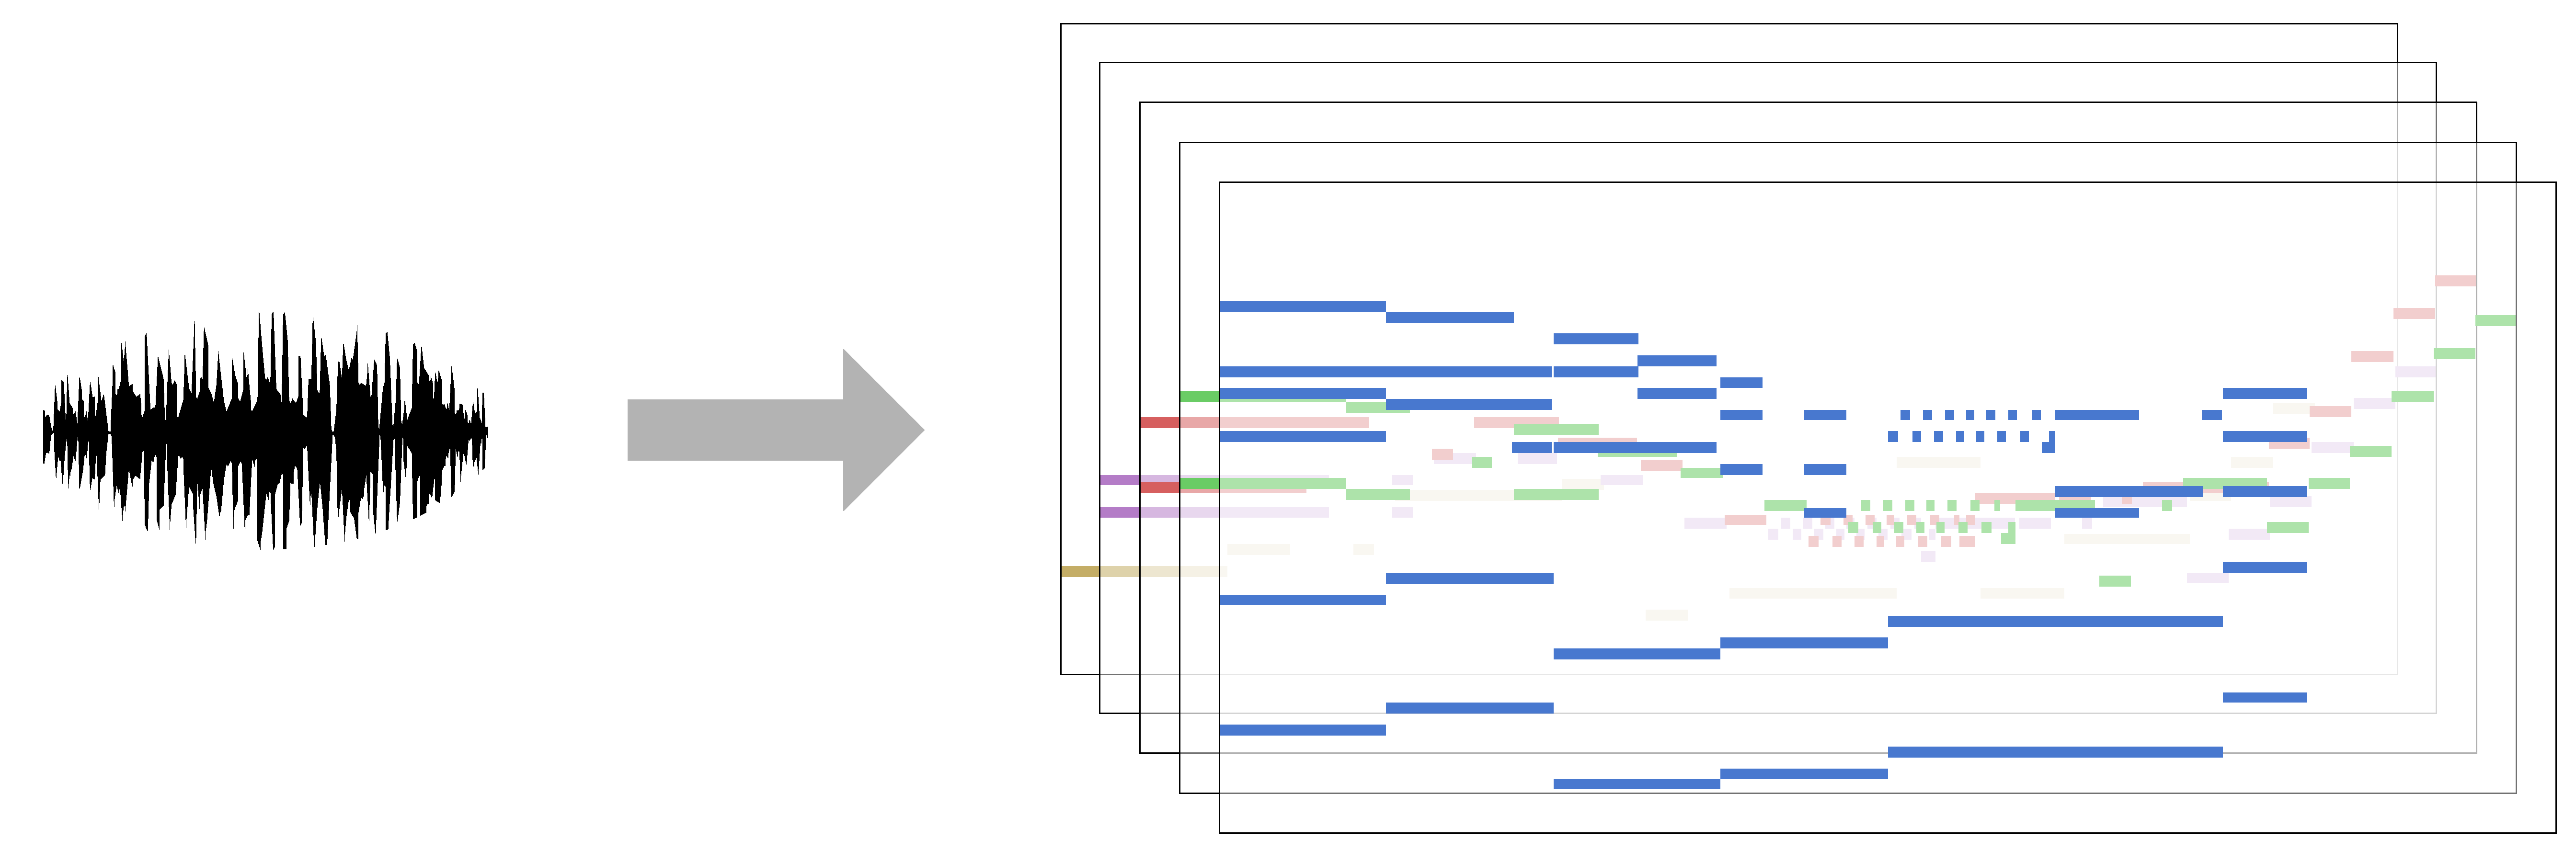
\includegraphics[width=\textwidth]{march-transcription.pdf}
	\caption{The automatic music transcription setup to be used in this thesis. Using per-instrument piano-roll representations is easier for machines to process, and avoids variability and subjectivity that may arise from symbolic and textual notations.} 
	\label{fig:transcription-to-piano-rolls}
\end{figure}

\emph{Automatic music transcription} (AMT) refers to an automated process that can identify musical events in the input audio and convert them into musical notations.
Historically, the definition of automatic music transcription varied by author, usually in terms of the form of the output representation.
In earlier works \cite{moorer1977transcription,piszczalski1977transcription}, the final output of the transcription system was to be the common music notation, i.e. a score, while later literature generalizes the problem by defining it as ``the analysis of an acoustic musical signal so as to write down the pitch, onset time, duration, and source of each sound that occurs in it" \cite{klapuri2006transcription} or ``the process of converting an acoustic musical signal into some form of musical notation" \cite{benetos2013amt}.
This thesis adopts per-instrument piano-rolls as the resulting representation of automatic music transcription, as shown in Figure \ref{fig:transcription-to-piano-rolls}, and defers the ``piano-roll to score" conversion as an out-of-scope task, which involves higher-level nontrivial tasks such as tempo and meter tracking, key signature detection, and music structure identification.
This can be justified since it allows the transcription model to focus on source separation and multi-pitch tracking, which are already highly challenging problems \cite{cemgil2006generative}.


To perform automatic music transcription, various properties of musical events, such as pitch, timbre, harmony, beats, etc., need to be defined and extracted from the audio.
In this sense, the setup of AMT is \emph{discriminative} in nature, meaning that it aims to identify different attributes from given audio, as opposed to \emph{generative} models concerning how to construct audio signals according to given conditions about those attributes.
Meanwhile, when a generative model is jointly trained with an encoder, it can learn to generate data samples from a small number of latent factors, while the encoder learns to extract those factors from the audio in a compact representation, as depicted in Figure \ref{fig:autoencoder}.
Since recently, with the increased capacity of machine learning models and hardware, many \emph{deep generative models} have been proposed and shown to be capable of processing high-dimensional multimedia data.
Furthermore, significant research efforts have been made toward learning disentangled representation of data, meaning that the latent factors contain meaningful information that can be easily separated and isolated.
To this end, the goal of this thesis is to study representation learning methods powered by deep generative models, accompanied with automatic generation of music, to obtain disentangled information from audio signals that can achieve better performance in music transcription.

\begin{figure}[t]
	\includegraphics[width=\textwidth]{autoencoder.pdf}
	\caption{A generative model has to know all of necessary information required to reconstruct the audio data, including pitch, timbre, loudness, and duration. Generative models can be jointly trained with an encoder that finds those semantic information, giving a transcriber-synthesizer pair; more detail on Subsection \ref{ch:deeplearning}.\ref{subsec:gan-encoder}.}
	\label{fig:autoencoder}
\end{figure}

\pagebreak

\section{Subproblems and Research Questions}\label{sec:subproblems}

This thesis concerns two major subproblems regarding the proposed approach toward automatic music transcription: 

\vspace{1em}

\begin{enumerate}
	\item Can we use generative methods to obtain disentangled representations of musical audio signals, to be used for automatic music transcription?
	\begin{enumerate}
		\item Can deep generative models such as \emph{generative adversarial networks} (GAN) learn to differentiate the concept of pitch and timbre, so that it can separately control them in its generation?
		\item How can we extend such generative model to work with arbitrary time scales, learning to encode and generate polyphonic notes with various onset times and durations?
		\item Can we make the latent representation used in the generative model convey information on the note-level events in the form of piano rolls, effectively performing music transcription?
	\end{enumerate}
	\item Can we build a music generation pipeline as a data augmentation tool which provides a large-scale representative dataset for training, in order to more effectively train the transcription model?
	\begin{enumerate}
		\item Can we use software instruments and audio post-processing techniques to span various timbres and recording environments that we are expected to encounter in transcription?
		\item How can we formulate a music language model that can be plugged into music synthesis and build generalizable datasets for polyphonic, multi-instrument music transcription?
		\item Would it be possible to incorporate the music generation pipeline into the deep generative model as a learnable component of the automatic music transcription algorithm?
	\end{enumerate}
\end{enumerate}

\vspace{1em}

The primary objective of this thesis lies on the first subproblem, concerning the disentanglement in representation learning on musical audio powerd by deep generative models.
Necessary to the successful application of data-driven learning is the availability of large-scale training data, while the difficulty of obtaining large-scale labeled data has always been a problem in music informatics.
The second subproblem is aimed at alleviating this issue by employing automatically generated datasets using software instruments and music language models.
In this sense, while not being the primary research objective of the thesis, effectively designing the data generation pipeline would be an indispensable component of achieving the primary goal.

\section{Definitions}\label{sec:definitions}

\paragraph{Research Areas}

\begin{itemize}
	\item \textbf{Music Information Retrieval (MIR)}: An interdisciplinary research area that concerns retrieving information from music.
	\item \textbf{Automatic Music Transcription}: An automated process of extracting musical events in the input audio and converting them into musical notations.
	\item \textbf{Multi-Pitch Estimation}: A task of estimating individual pitch values in polyphonic music. Synonymous with \textbf{Multiple Fundamental Frequency (F0) Estimation}.
\end{itemize}

\noindent 
\paragraph{Music and Audio Signal Processing}

\begin{itemize}
	\item \textbf{Pitch}: A perceived quality of highness or lowness of a sound that is closely related to the fundamental frequency.
	\item \textbf{Spectrogram}: A two-dimensional representation of an audio signal that visualizes the spectral decomposition of the sound over time, using the magnitudes of the short-time Fourier transform (STFT).
	\item \textbf{Short-Time Fourier Transform (STFT)}: A linear transformation that maps a one-dimensional signal to a two-dimensional representation that contains the Fourier spectra of the short-time segments.
	\item \textbf{Music Language Model}: Modeling of symbolic sequences of music.
\end{itemize}

\paragraph{Machine Learning and Deep Learning}

\begin{itemize}
	\item \textbf{Heuristics}: A method that is not optimal or perfect but useful for immediate practical purposes, usually employing manually designed functions or computations.
	\item \textbf{Data-Driven Method}: A method based on the optimization of model parameters using examples of data.
	\item \textbf{Ground-Truth}: Annotations corresponding to the data examples that are assumed to be true.
	\item \textbf{Machine Learning}: Programming computers to learn from experience, without being explicitly programmed \cite{samuel1959ml}.
	\item \textbf{Supervised Learning}: A category of machine learning methods that require labeled training data.
	\item \textbf{Unsupervised Learning}: A machine learning task to discover the hidden structures from unlabeled data.
	\item \textbf{Deep Learning}: A family of machine learning methods that employ multiple layers of learned representations, obtained by composing simple transformations at each level \cite{lecun2015deeplearning}.
	\item \textbf{Representation Learning}: A task of learning the underlying representations of data that make it easier to extract useful information \cite{bengio2013representation}.
	\item \textbf{Generative Model}: A model that is capable of generating data points that are coherent to supplied training examples.
	\item \textbf{Disentanglement}: A desirable quality of a learned representation from which meaningful information can be easily separated and isolated.
\end{itemize}

\section{Delimitations/Limitations}\label{sec:limitations}

Because of the sophisticated and open-ended nature of automatic music transcription, it is necessary to define the scope of the tasks and data that this thesis will be concerned with.
The purpose of this section is to define those limitations in terms of the scope of music that the proposed AMT system can process, the required capability of symbolic music processing, and the need for the perceptual studies regarding the validity of AMT systems.


\subsection{Scope of Music}

Music signals typically contain both harmonic and percussive sources. 
In the signal processing point of view, harmonic sounds are periodic and contains energy only at certain frequencies usually at the multiples of the fundamental frequencies, whereas percussive sounds have continuous frequency spectra in which it is not possible to define a fundamental frequency.
Consequently, transcription models for harmonic sounds and percussive sounds require different techniques according to their nature.


This thesis will limit the focus on the transcription of harmonic sounds and therefore use the per-instrument piano roll notation (Figure \ref{fig:transcription-to-piano-rolls}) as the output representation.
This is a realistic trade-off to make, because of a number of reasons.
First, learning to simultaneously model the harmonic and percussive sounds is a harder problem both conceptually and computationally.
Secondly, it is possible to plug a harmonic-only model into a pipeline consisting of HPSS (harmonic-percussive source separation) and a percussion transcription model as an alternative to the comprehensive approach.
Lastly, polyphonic transcription is considered to be the most difficult problem in the domain of automatic transcription, and it is sensible to tackle this as a standalone problem in a simplest possible setup.
Excluding percussive sounds will disallow using most of pop music tracks as-is, but multi-track datasets can still be utilized since they contain each track separately.


Additional limitations should be considered on the types of the instruments and their sound variations.
Depending on the instrument, the same line segment in a piano roll representation may contain a variety of musical techniques, such as vibrato, tremolo, pizzicato, and the usage of a mute or harmonics, among others.
In order to accurately produce the piano roll transcription that is invariant to those variations, the model has to be trained to classify them as nonessential information, requiring the availability of the dataset with the annotations for those techniques.
While an ideal model should learn those concepts as humans do, too much timbral or temporal variation for an instrument will prevent the model from learning a consistent representation corresponding to the instrument.
Therefore, for the immediate purpose of this thesis, a dataset that does not contain too much variations will be employed, similarly to the pilot study which used non-vocal harmonic sounds of Western classical instruments.


\subsection{Symbolic Processing of Notes}

As mentioned and justified in the statement of problem (Section \ref{sec:statement}), by choosing per-instrument piano rolls as the output of transcription, many structure-level and symbolic-level concerns in music transcription are excluded from the scope of this study.
The difference between the piano roll output and the full human-readable score output becomes apparent when we compare the piano rolls in Figure \ref{fig:transcription-to-piano-rolls} with Figure \ref{fig:wedding-march-score}, which is the original score from which the piano rolls are plotted.
There are many aspects in producing the score output that are highly subjective and difficult to derive a consistent evaluation metric from, such as the interpretation of legatos or staccatos and the aesthetic choices for typesetting, providing an additional justification for using the piano roll notation.


The MIDI file format is suitable for conveying the data equivalent to per-instrument piano rolls, consisting of multiple tracks of \texttt{note\_on} and \texttt{note\_off} events with the corresponding timestamps.
MIDI will therefore be the output format of the proposed AMT system, which can also be conveniently played back by media player software.
Music typesetting software such as Sibelius or Finale can render a MIDI file into a score notation using the metadata in the file as well as some heuristics for quantization, however the readability of the score rendered from a transcribed MIDI file would be limited, due to imperfect transcription and the absence of metadata on the time and key signature.


\begin{figure}
	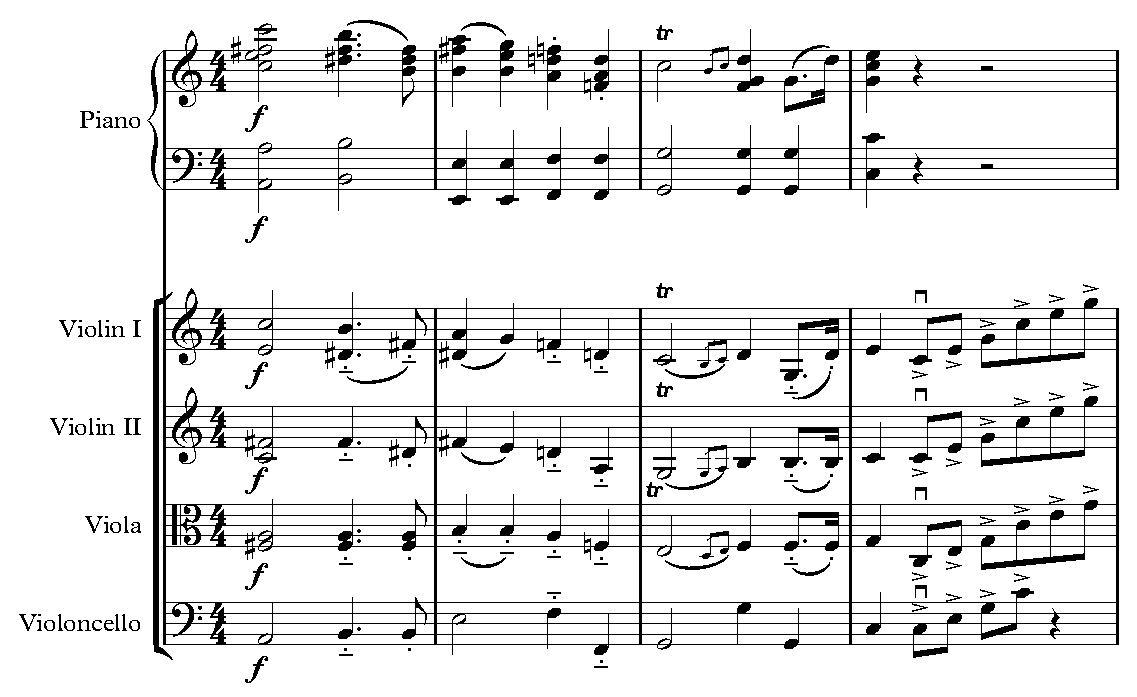
\includegraphics[width=\textwidth]{march-score.pdf}
	\caption{The full score notation of the music used to build the piano rolls in Figure \ref{fig:transcription-to-piano-rolls}. To fully recover this level of notations from the audio, the transcriber has to make many additional decisions than for the piano rolls, such as determining the key signature, time signature, clefs, dynamics, trills, bowing instructions, etc.}\label{fig:wedding-march-score}
\end{figure}



\subsection{On the Need for Perceptual Studies}

This study of automatic music transcription is entirely quantitative and does not involve subjective tests on human participants.
The dataset to be used in thesis consists of audio signals, i.e. waveforms encoding the physical vibrations of air.
However, music is essentially a perceived notion, and thus are the core qualities of sound --- pitch, timbre, and loudness --- which are the output of automatic transcription.
For this reason, manually annotating polyphonic music is an error-prone process, where any two annotators may produce drastically different annotations.
Although this problem of inaccuracy and subjective difference is often overcome by using a ground-truth dataset synthesized from known frequency information, the gap still persists between what a model can learn from synthesized audio and what it will respond to the real-world sound.
This thesis aims to take one step further than using synthesized training datasets, by building a generative model that can better model the real-world sound of interest.

The goal of automatic transcription is at a lower level than the tasks like chord recognition and melody tracking, which may incur even more subjective disagreements caused by the imprecise definitions of chords and melodies.
Pitch is relatively precisely defined in this sense, and formulating automatic music transcription as an audio-to-piano-roll conversion mostly eliminates the ambiguity that exists in chord recognition and melody tracking.
There exist some cases where the mathematical definition of fundamental frequency still cannot be applied for all pitched sounds, such as the Shepard tone \cite{shepard1964circularity} where the pitch of a harmonic sound fails to be consistently mapped to a fundamental frequency.
However, disregarding these few edge cases, this study assumes that the piano roll notation can convey an objective transcription for practical purposes, postulating AMT as a mathematical problem which does not require experiments on human subjects.


\subsection{The Ultimate Goal of Automatic Music Transcription}

Finally, a consideration is needed for the fundamental limitation on any music transcription task, either automatic or manual, and when it can be said that AMT is solved.
Polyphonic music contains a mixture of sounds with an indefinite number of notes being played simultaneously; even the most experienced musicians may not be able to identify every note, and the audio mixture may not contain the sufficient information to convey all notes in the first place.
It would be unreasonable to expect anyone to perfectly transcribe all notes in the score of an orchestral music from an audio file, but it would be sensible for a trained musician to produce a version of score that, when played by the same orchestra, sounds indistinguishable to the original recording.
Considering these limitations, passing this ``transcriptional Turing test'' as shown in Figure \ref{fig:turing}, rather than achieving the 100\% accuracy on a certain dataset, should be the ultimate goal of automatic music transcription, at which point it can be said to have a human-level intelligence on this task.

Developing an AMT algorithm that can pass this test is not a goal of this thesis, because the performance of AMT is far behind the human performance.
Therfore, this thesis pursues a more tangible goal of achieving a better accuracy in transcribing music that is easy enough for human transcribers but challenging for machines.
More details on the dataset and the evaluation method are provided in Chapter \ref{ch:methods}. \TODO{FIX}


\begin{figure}
	\includegraphics[width=\textwidth]{turing.pdf}
	\caption{The \emph{transcriptional Turing test}, to test whether an automatic music transcription algorithm has reached human-level. While this provides some conceptual insights to the adversarial training setup, to be covered in the later chapters, fully achieving the human-level performance is out of scope of this thesis.}
	\label{fig:turing}
\end{figure}

\pagebreak

\section{Need for Study}

The nature of music transcription is multifold; to create a complete transcription, one has to identify all instruments, onsets, dynamics, and the pitch traces for every instrument present in the music, and it is still far from achieving the human-level accuracy.
The need for study arises naturally, not only because this is an intriguing problem in the interdiscipline of music and technology that has remained unsolved for decades, but also because the solution to this problem can provide practical benefits to many applications.

In order to bolster the need for this study, this section starts by introducing such applications, followed by discussions on the advantages of employing generative models as a means of better capturing musical semantics and a new paradigm of MIR research.
A brief perspective on AMT is presented in the context of wider AI research, followed by the organization of the chapters.


\subsection{Applications of Automatic Music Transcription}\label{sec:applications}

Many applications of the techniques in the realm of automatic music transcription is on interactive music systems.
\citeA{vercoe1984performer} proposed a quest for a \emph{synthetic performer}, which can listen, perform, and learn in the context of live performance, and automatic \emph{real-time accompaniment} \cite{dannenberg1985accompaniment} based on dynamic programming was one of the first successful demonstrations of AMT techniques.
\emph{Score following} is a general term referring to the synchronization of a computer with a performer playing a known score \cite{orio2003following}.
An offline music-to-score matching algorithm can also be applied to intelligent audio editors \cite{dannenberg2003following}.

Music recommender systems can combine many kinds of information for improved music retrieval and personalization \cite{celma2010music}.
Content-based music recommender systems can utilize not only the metadata but also the audio content, and methods using timbral \cite{magno2008recommendation}, temporal \cite{li2007recommender}, and tonal features \cite{lu2009recommendation} have been introduced.
These music recommender systems can be further improved when the complete information on each domain is made available through AMT.

AMT system can help create the database for query-by-humming \cite{ghias1995humming} by automatically creating melody annotations, where users can retrieve music by humming an excerpt of the song.
Such database can also facilitate a large-scale musicological analysis \cite{abdallah2015british}, as well as the development of computer-aid music composition \cite{agostini2013aid} that incorporates musicological knowledge.


\subsection{Generative Modeling for Fully Capturing Semantics}

Being ``generative'' means that a model is capable of generating new samples in the domain of the original data.
Generation in the symbolic domain creates new musical scores, and a generative model in the audio domain creates audio waveform.
These two kinds of generative systems are familiar to computer music artists and are referred to as algorithmic composition \cite{fernandez2013ai} and sound synthesis \cite{cook2002synthesis} models.
This thesis defines the term ``generative model'' more specifically, as a model that can learn the distribution of provided data and can sample new samples in the original distribution.
This differs from the term ``generative'' used in computer music in a sense that it aims to accurately model and learn to regenerate the real-world audio to be used in music transcription, rather than focusing on artistic aspects of generating new kinds of sounds and music.

By learning to generate data using fewer parameters than the scale of the dataset, a model has to discover the underlying natural features from the distribution of data.
In music transcription, these features correspond to the musical concepts such as pitch, timbre, and rhythm.
This idea follows what Richard Feynman once wrote on his blackboard, \emph{``What I cannot create, I do not understand''} and \emph{``Know how to solve every problem that has been solved''}.
He meant that the marker for truly understanding something is the ability to construct it completely from scratch.
Generative models are a branch of unsupervised learning, because it does not require labeled data.
\citeA{lecun2016unsupervised} introduced unsupervised learning as a cake, comparing supervised learning as icing and reinforcement learning as the cherry on the top, by which he meant that generative model needs to predict much larger scale of information but is able to learn the ``common sense''.

\begin{figure}
	\includegraphics[width=\textwidth]{generative-evolution.pdf}
	\caption{Increasingly realistic qualities of the generated faces using generative adversarial networks as shown in \protect\cite{brundage2018malicious}; images are from \protect\cite{goodfellow2014gan}, \protect\cite{radford2015dcgan}, \protect\cite{liu2016cogan}, and \protect\cite{karras2017pggan}.}
	\label{fig:generative-evolution}
\end{figure}


Inherently, unsupervised learning is less well-defined than supervised learning, and this is the reason why unsupervised learning is sometimes synonymous with clustering, because finding clusters is usually as much an unsupervised learning system can do.
However, a recent success of deep learning introduced a new breed of generative models, enabling an end-to-end generation of complex data such as photos and audio signals.
\emph{Generative adversarial network} (GAN) \cite{goodfellow2014gan} is the most notable among them, and its performance in generating realistic images has been improving at an extraordinary pace, as shown in Figure \ref{fig:generative-evolution}.
Combined with the various techniques for manipulating the semantic information in GANs as will be introduced in Section \ref{ch:deeplearning}.\ref{sec:gan}, this hints at a completely new kinds of generative methodologies for audio processing.


In this context, this thesis aims to design and develop improved methods for automatic music transcription with a deeper understanding of musical semantics powered by deep generative models.
The idea specifically hypothesizes that by training a generative model, it is possible to learn disentangled representations, from which the information necessary for transcription can be easily extracted, as depicted in Figure \ref{fig:autoencoder}.
By doing so, the ultimate objective is to build an end-to-end differentiable model that connects the piano roll representation to audio signals, in order to perform automatic music transcription --- obtaining the most likely piano roll representation for given audio.


\subsection{Generative Models as a new Paradigm of MIR Research}

\begin{figure}
	\begin{subfigure}[b]{\textwidth}
		\centering
		
\includegraphics[width=0.75\textwidth]{paradigms-1-manual.pdf}
		\caption{A traditional rule-based model based on hand-crafted features.}
		\label{}
	\end{subfigure}
	\begin{subfigure}[b]{\textwidth}
		\centering
		\vspace{1em}
		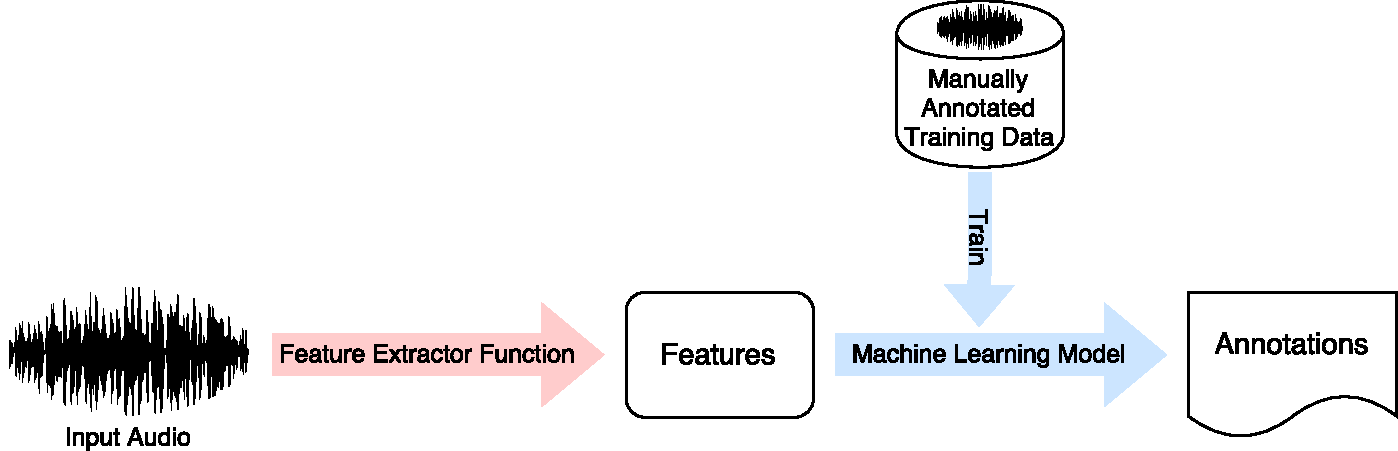
\includegraphics[width=0.75\textwidth]{paradigms-2-features.pdf}
		\caption{A data-driven machine learning model built upon hand-crafted features.}
		\label{}
	\end{subfigure}
	\begin{subfigure}[b]{\textwidth}
		\centering
		\vspace{1em}
		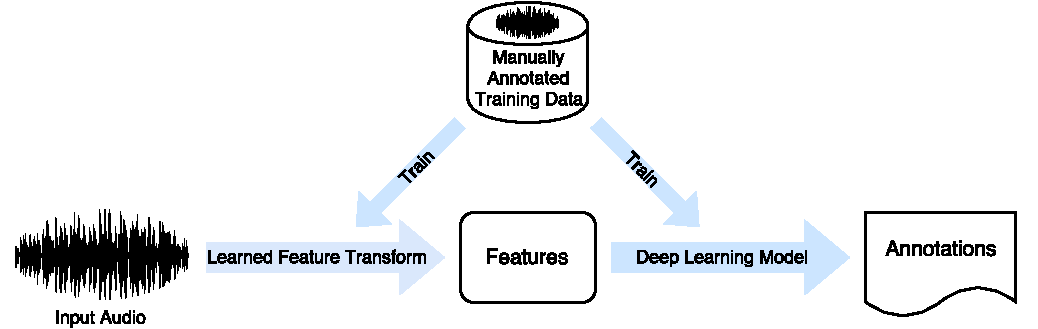
\includegraphics[width=0.75\textwidth]{paradigms-3-end-to-end.pdf}
		\caption{An end-to-end data-driven model without manual feature engineering.}
		\label{}
	\end{subfigure}
	\begin{subfigure}[b]{\textwidth}
		\centering
		\vspace{1em}
		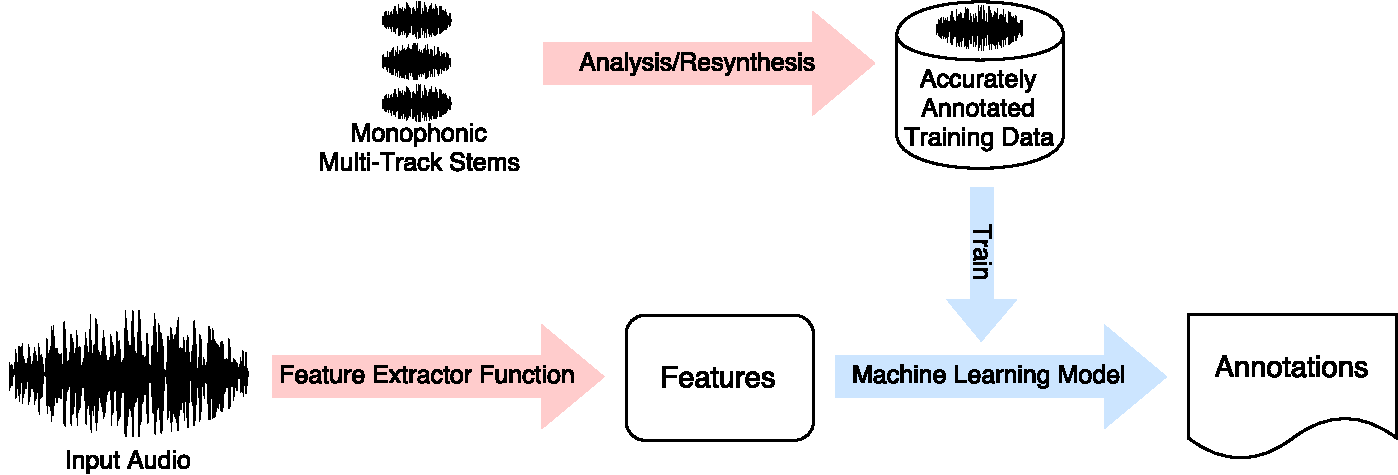
\includegraphics[width=0.75\textwidth]{paradigms-4-analysis-synthesis.pdf}
		\caption{Analysis/synthesis \cite{salamon2017analysis} for accurate and automatic annotation.}
		\label{}
	\end{subfigure}
	\begin{subfigure}[b]{\textwidth}
		\centering
		\vspace{1em}
		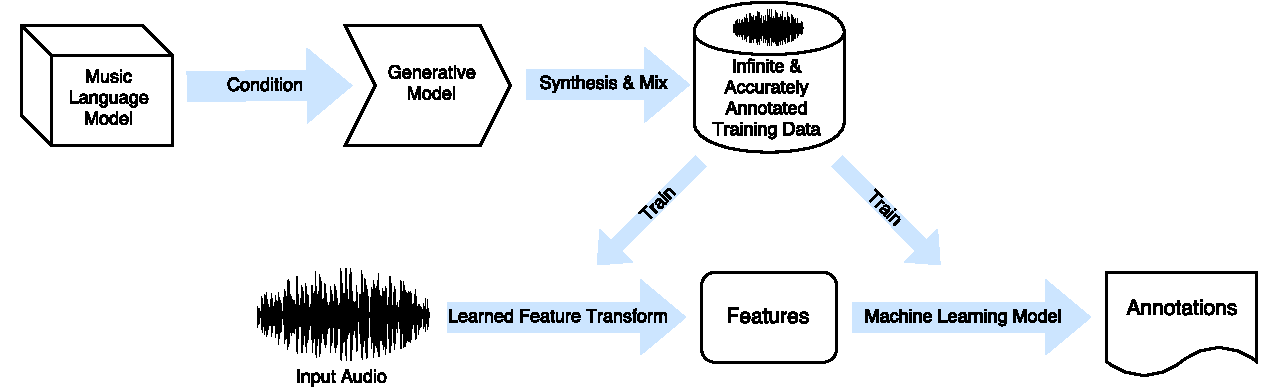
\includegraphics[width=0.9\textwidth]{paradigms-5-proposed.pdf}
		\caption{The proposed setup, leveraging the music language model and the generative model providing an infinite source of accurately annotated training data.}
		\label{}
	\end{subfigure}
	\caption{Paradigms of MIR research. Blue arrows indicate learnable components.}
	\label{fig:paradigms}
\end{figure}


The second subproblem stated in Section \ref{sec:subproblems} considers data generation as an augmentation tool for further improving the performance of an AMT system.
In the proposed setup, a music language model is trained to produce meaningful symbolic music sequences to be fed to the generative model, which can synthesize multi-track polyphonic music along with the corresponding annotations.

This architecture can be aligned with the previous paradigms of MIR research, as shown in Figure \ref{fig:paradigms}:
(a) The earlier methods typically use a carefully crafted function to extract features and performed rule-based predictions, whereas (b) the data-driven methods replace the later part with a machine learning model trainable with a dataset.
(c) With the access to a larger amount of data and deep learning techniques, end-to-end models eliminate the need for manually designed feature extractors by learning the feature transform directly from data.
(d) The analysis/synthesis model \cite{salamon2017analysis} overcomes the data scarcity problem by automatically generating annotations from multi-track stems, to be supplied to a polyphonic transcription model.
A shortcoming of this approach is that it requires a multi-track dataset composed of monophonic stems.
(e) The proposed setup extends the analysis/synthesis model by building a fully learnable pipeline, where the synthesizer component of the generative model serves as an effectively infinite source of labeled training examples.

In theory, this can constitute a positive feedback loop where data augmentation improves the performance of the transcription model, and the improved synthesizer component of the transcription model provides better data augmentation.
Another advantage of this setup is that the data augmentation pipeline is not limited to training an AMT model but applicable to any music information retrieval tasks.

\subsection{In the Broader Context of Machine Listing in AI Research}

Using generated audio data and generative models is partly motivated by the fact that synthesized music is more prevalent and perceptually more familiar to people than synthesized texts or pictures, considering that many commercial music tracks are often produced entirely using software instruments, except for the vocal parts.
This suggests that synthesized and generated audio may more accurately model the distribution of the real audio data to be transcribed.
This generative approach also aligns well with how actual musicians transcribe music, where they match given audio with their knowledge of how the instruments sound when played in a certain combination of rhythms and melodies.
Therefore it is reasonable to claim that machines should also be able to perform in a similar way, provided that a proper representation of knowledge about the music and instruments is available.

The task of automatic music transcription shares many common values with other machine learning tasks, such as image segmentation, machine translation, and speech recognition, in a sense that the core task is to build an intelligent system that can extract and process semantics that are conveyed in complex signals.
This is an essence of artificial intelligence (AI)
--- a system that perceives its environment and takes actions that maximizes the utility \cite{russell2009ai} --- 
where an intelligent system has to understand the semantics of complex data coming from the environment in order to perform well in its tasks.
To this end, the problem of automatic music transcription is not just an intriguing task in music technology, but will also be a key component of the AI-enabled future society, constituting a musical brain of AI in the form of advanced machine musicianship \cite{rowe2003musicianship}.


\subsection{Organization of Thesis}


To summarize, this thesis considers the possibility of using deep generative models to learn the musical concepts necessary for automatic music transcription, as well as using the learned generative component as an augmentation tool for further improving the performance of the transcription model.

There exists a rich history of research aiming at understanding of musical sounds and automatic music transcription, and to validate this claim as a feasible research direction and place this proposal in the context of this continuum of research, Chapter \ref{ch:mir} provides a review of the standard methods and the current state of the art of automatic music transcription research.
%One of the most exciting phenomena that have been happening in the field of machine learning during the past five years is the advent of deep learning and its tremendous success in computer vision, natural language processing, and many other fields.
%The success was made possible by the unprecedented scale of high-performance computing resources that became available, which made intelligent systems capable of processing machine learning algorithms and data pipelines that were infeasible to be realized just until a few years ago.
%At the same time, a number of new models and techniques have been devised to drastically improve the effectiveness and flexibility of existing algorithms.
Because it is expected that the techniques of deep learning will play the most important role in this study, a general introduction to deep learning and deep generative models is provided in Chapter \ref{ch:deeplearning}, with a focus on generative adversarial networks, which are by far the most capable family of deep generative models.


Chapter \ref{ch:methods} presents the tentative design of the proposed automatic music transcription research, along with the architecture of the deep generative model and the datasets to be used.
%The pipeline incorporates deep learning and music signal processing methods as well as other important components including data augmentation, software instruments, audio synthesis, and music language models.
Subsequently, some results of the preliminary experiments in this direction of research are introduced in Section \ref{ch:pilot}, including a monotonic pitch estimator based on time-domain convolutional neural network and a generative adversarial network trained on log-magnitude spectrograms of instrument note samples.

\setcounter{chapter}{1}
%!TEX root = ../dissertation.tex
% this file is called up by thesis.tex
% content in this file will be fed into the main document

%: ----------------------- introduction file header -----------------------
% the code below specifies where the figures are stored
\graphicspath{{2-mir/figures/}}

\chapter{Music Information Retrieval for Transcription}
\label{ch:mir}

Being able to accurately identify all musical events from audio and transcribe them into musical notations is an essential skill for musicians as well as a paramount goal of music machine learning research.
Enabling an automatic conversion between musical audio and symbolic notations, automatic music transcription opens up many new possibilities, including the applications listed in Subsection \ref{ch:introduction}.\ref{sec:applications}.


Due to the complexity and difficulty of creating a completely end-to-end music transcription system, many existing approaches focus on a specific subtask of the problem \cite{casey2008mir}, e.g. extracting onsets and beats, recognizing timbre and instruments, tracking monophonic and polyphonic pitches, or separating audio sources from a mixture.
Each of these subtasks poses interesting goals and applications even without the lofty goal of end-to-end music transcription, which are subproblems of \emph{music information retrieval} (MIR).
Although this term has existed since 1960s \cite{kassler1966mir}, it was only after the late 1990s when active research on this area has spun off from computer music and computational musicology literature.
During the last two decades, numerous sophisticated and novel approaches for each of these subproblems have been introduced, that have continuously improved the performance in terms of the accuracy in predicting the correct annotations.
This chapter starts by introducing the standard pipeline of music information retrieval that are commonly employed in most MIR models and reviews the state-of-the-art techniques in each area relevant to music transcription.
The purpose of this chapter is not to provide an all-encompassing survey over the history of MIR research but to show a clear common pattern over the areas of MIR where the machine learning models have been evolving from simple heuristics based on hand-crafted features to sophisticated deep learning models with millions of parameters.
Many methods employing deep neural networks are referenced in this chapter, and the concepts and the formulation of those models such as convolutional newral networks (CNN) and recurrent neural networks (RNN) are described in Chapter \ref{ch:deeplearning}.


\section{The Standard Pipeline}

Audio data is huge in volume; a typical audio track contains 44,100 real-numbered samples per second, and sometimes even more.
Therefore, computational methods for extracting musical information from audio usually contains a pipeline of feature extraction stages to reduce the volume and increase the interpretability of input data, as shown in Figure \ref{fig:pipeline}.
The pipeline includes a few techniques widely used in speech processing, as well as many feature extraction stages created for music-specific purposes.

\begin{figure}[t]
	\includegraphics[width=\textwidth]{pipeline.pdf}
	\caption{\small The standard pipeline for music feature extraction. An appropriate set of feature extraction methods needs to be heuristically selected depending on the task.}\label{fig:pipeline}
\end{figure}

While there are many MIR tasks that operate on the track level, such as music recommendation, tagging, and genre classification, most subtasks of music transcription involve the prediction of labels that are dependent on time, operating either in the sample-level or frame-level.
Frames are created by taking a series of overlapping short-time audio segments, where the length of a segment typically ranges from 10 to 50 milliseconds, and optionally multiplying them by a windowing function.
Taking discrete Fourier transforms on the frames produces a \emph{short-time Fourier transform} (STFT), and the magnitude of an STFT gives a \emph{spectrogram}.
Spectrograms give very rich information about the audio; for example, the contour of melodies and the dynamics of music are usually identifiable from the spectrogram image.
Spectrograms are expressive enough to be used as an output of sound synthesis or a source separation algorithm, and the corresponding audio signals can be reconstructed without incurring significant perceptual inconsistencies \cite{griffin1984lim, leroux2010spectrogram}.
However, the dimensionality of a spectrogram is still quite high, making it computationally prohibitive to run many algorithms directly on an STFT or a spectrogram.
This necessitated further transformations by the means of filterbanks, such as \emph{Mel-Frequency Cepstral Coefficients} (MFCC) \cite{logan2000mfcc} by applying the Mel filterbank inspired by the human auditory perception and taking the first few DCT components that contain independent factors describing the spectral shape.
\emph{Constant-Q transform} (CQT) \cite{schorkhuber2010cqt} uses a filterbank where the center frequencies of filters have a constant Q factor, which is the ratio between the center frequency and the 3 dB bandwidth of a filter.
By configuring CQT to produce 12 filters per octave, it is possible to obtain the coefficients corresponding to each musical tone, and to fold the representation to produce a \emph{chromagram} \cite{harte2005chromagram}.
To extract the beat and tempo information, a heuristic function, such as the first-order difference of the time-domain log energy function or the \emph{spectral flux} that measures the total energy increase over the STFT frequency bins, is applied to formulate a novelty curve.
This curve can then be used to measure energy bursts that are typically present in the onsets of notes \cite{bello2005onset}.
The onset information can be further processed to obtain tempo information via \emph{tempogram} \cite{cemgil2000tempogram} or cyclic tempogram \cite{grosche2010tempogram}.


Once an appropriate set of features are obtained, the next steps for MIR algorithms typically involve applying a classification model.
Examples include Random forests, support vector machines (SVM), and Gaussian mixture model (GMM) classifiers that have been applied to music tagging \cite{ness2009tag}, melody extraction \cite{bittner2015contour}, and genre classification \cite{tzanetakis2002genre} tasks.
Hidden Markov models (HMM) are widely employed for modeling sequence data such as chord progressions \cite{cho2010chord} as well as to smooth the sequence output as a post-processing step \cite{khadkevich2009hmm}, often paired with Gaussian mixture models as the emission probability distribution.
Since finding a better feature representation played a crucial role in earlier MIR systems, many approaches focused on engineering sophisticated feature transformations \cite{harte2006tonnetz} and devising clever pre- and post-processing steps \cite{oudre2009chord}.


More recent approaches have successfully eliminated some or all feature transformation stages in the standard MIR pipeline by training a deep model to learn the feature from the spectrogram or audio waveforms.
Applications of deep learning arose in virtually all types of MIR tasks, including melody extraction \cite{bittner2017deepsalience}, beat tracking \cite{vogl2017drum}, and genre classification \cite{oramas2017genre}.
Apart from a small number of end-to-end approaches, most deep learning models for music still rely on predefined feature transforms such as STFT or CQT, because those features make it easier for a model to learn meaningful concepts without overfitting, using a smaller amount of parameters and thus using less powerful hardware.
%In theory, however, any feature extraction stage induces a loss of information, and it suggests that the best-performing model would benefit most from the raw audio data.

Having covered the general approaches in MIR, the following sections provide more in-depth literature reviews on the different subtasks relevant to automatic music transcription, starting from the simplest problem of monophonic picth tracking.


\section{Monophonic Pitch Tracking}\label{sec:monophonic}

Estimating the fundamental frequency (f0) of a monophonic audio signal, also known as pitch tracking or pitch estimation, is one of the simplest but a long-standing topic of research in audio signal processing.
Pitch estimation plays an important role outside of automatic music transcription as well, where monophonic pitch tracking can be used as a method to generate pitch annotations for multi-track datasets \cite{bittner2014medleydb} or as a core component of melody extraction systems \cite{bosch2014melody, mauch2015computer}.

%Pitch is defined as a subjective quality of perceived sounds and does not precisely correspond to the physical property of the fundamental frequency \cite{hartmann1997signals}.
%However, apart from a few rare exceptions, pitch can be quantified using fundamental frequency, and thus they are often used interchangeably outside psychoacoustical studies. 
%For convenience, the two terms are interchangeably throughout this chapter.

Computational methods for monotonic pitch estimation have been studied for more than a half-century \cite{noll1967cepstrum}, and many reliable methods have been proposed since.
Earlier methods commonly employ a certain candidate-generating function, accompanied by pre- and post-processing stages to produce the pitch curve.
Those functions include the cepstrum \cite{noll1967cepstrum}, the autocorrelation function (ACF) \cite{dubnowski1976acf}, the average magnitude difference function (AMDF) \cite{ross1974amdf}, the normalized cross-correlation function (NCCF) as proposed by RAPT \cite{talkin1995rapt} and PRAAT \cite{boersma1993praat}, and the cumulative mean normalized difference function as proposed by YIN \cite{decheveigne2002yin}. More recent approaches include SWIPE \cite{camacho2008swipe}, which performs template matching with the spectrum of a sawtooth waveform, and 
pYIN \cite{mauch2014pyin}, a probabilistic variant of YIN that uses a Hidden Markov Model (HMM) to decode the most probable sequence of pitch values.
According to a few comparative studies, the state of the art is achieved by YIN-based methods \cite{von2010comparison, babacan2013comparative}, with pYIN being the best performing method to date \cite{mauch2014pyin}.

While these methods work well for monophonic audio, it is not enough for general music transcription, where multiple concurrent notes and sound sources are present.
To address this situation, the next section reviews the techniques for tracking multiple pitches.


\section{Multiple Fundamental Frequency Estimation}

Among the subtasks of automatic music transcription, estimating the pitch from polyphonic recording poses the most difficult challenges, as apparent from the recent stream of results from MIREX challenges \cite{downie2014mirex}.
The task is commonly referred to as \emph{multiple fundamental frequency estimation} (Multi-F0 estimation, or MFFE) and is in some sense a superset of the onset and beat detection problems as well as chord and melody tracking problems,
since the frequency tracking task has to indicate the onset and offset of every sound, and tracking chords and melodies becomes much easier when the correct annotations for all pitch contours are available.

Many early methods for MFFE \cite{klapuri2003multiple} focused on extracting features like harmonicity and spectral smoothness from the audio spectrogram and devising a good heuristic for frequency estimation.
Another major technique for polyphonic music transcription is \emph{non-negative matrix factorization} (NMF) \cite{lee2001nmf}, based on the assumption that the spectrogram is a low-rank matrix which is a multiplication of the harmonic profile of each notes and the note activation patterns.
While some approaches \cite{gao2017nmf} based on NMF performs close to the state of the art, it has a drawback of having to obtain duplicate pitch templates for multiple instruments \cite{bertin2010nmf}.
Other data-driven approaches include probabilistic models based on dynamic Bayesian networks \cite{raczynski2013dynamic} and hierarchical graphical models \cite{pesek2017hierarchical}, and deep learning models using convolutional neural networks \cite{bittner2017deepsalience}, recurrent neural networks \cite{bock2012rnn,sigtia2016endtoend}, and most recently an architecture combining convolutional and bidirectional recurrent neural networks \cite{hawthorne2018piano}.

With the state of the art nearing the perfect accuracies \cite{ewert2017transcription} on the MAPS dataset \cite{emiya2010multipitch} which have been the standard evaluation dataset for piano transcription algorithms, more systematic assessments of transcription models have recently been proposed.
These include the study of invariance under data augmentation \cite{thickstun2017invariances} and the entanglement of note representations that may prevent accurate predictions for unseen combinations of notes \cite{kelz2017entanglement}.

In \cite{li2017infinite}, the idea of using on-the-fly synthesized training dataset for piano transcription was explored, using a simple fully-connected neural network operating on the CQT representation.
The idea of using generative models to predict multiple fundamental frequencies is also not new \cite{dubois2005harmonic,cemgil2006generative}, but they relied on manually designed generative models for sound generation, which might have led to poor generalizability.
Using deep generative models is expected to help overcoming this limitation, since deep learning methods is known to be excellent in learning embeddings and manifolds that are generalizable to different tasks and domains.


\section{Source Separation and Music Translation}\label{sec:separation}

Source separation refers to the task of separating sound sources from a mixture signal, and is closely related to automatic music transcription, because it provides a means to separate each instrument sources from multi-instrument music.
This problem is also called as a \emph{cocktail party problem}, based on humans' ability to focus on a single voice at a noisy cocktail party.
Sound source separation has been a popular research topic since the seminal work on \emph{auditory scene analysis} by \citeA{bregman1990asa}, from which stemmed computational auditory scene analaysis (CASA) \cite{brown1994casa}, a problem of using computational models to analyze an auditory scene, identifying the sources and location of all nearby sounds.
In this sense, automatic music transcription and sound source separation are particular aspects of auditory scene analysis \cite{plumbley2002transcription}, and source separation enables similar kinds of applications to AMT, such as music editing, 3D sound rendering, and information retrieval systems.


\emph{Blind source separation} refers to the situation where no information about the sources or the mixing process is known \cite{bell1995blind}, whereas \emph{informed source separation} \cite{vincent2013separation} concerns the case where some level of side information is available, e.g. the presence of a score \cite{ewert2014separation}.
Blind sound source separation has to resort to using purely statistical approaches such as indepenent component analysis \cite{saruwatari2006ica} or robust PCA \cite{huang2012separation}, whereas informed source separation can leverage the knowledge on the musical structure \cite{rafii2013separation, liutkus2012separation} or the timbral differences of the sources \cite{li2007separation,ono2010hpss} for better separation.
Probabilistic models for source separation \cite{ozerov2007separation,leglaive2016prior} have also been developed, and source-filter modeling \cite{heittola2009separation,durrieu2011separation} is a generative approach which separately models a source that creates a sound and a filter that shapes the timbre.
The proposed AMT model is similar to source-filter models in a sense that it describes the generative process of each sound, but also relates to timbre-informed source separation models \cite{miron2018thesis}, because it needs to learn the concept of timbre to produce per-instrument piano rolls.


A closely related problem to source separation is audio translation, which concerns mapping input audio to a corresponding output with some desired properties, such as speech with reduced noise, singing voice separated from music, or the same speech content in the voice of a different speaker.
\citeA{barry2018style} applied the style transfer algorithm \cite{gatys2015style} to an ensemble of STFT, CQT, and Mel spectrograms, to transfer musical styles capturing harmonic, rhythmic, and timbral elements.
The \emph{U-Net} architecture \cite{ronneberger2015unet} uses an encoder-decoder framework with skip connections between the hidden layers at the same level of abstraction to perform image translation, and a singing voice separation model can be trained using this architecture \cite{jansson2017separation}.
The encoder-decoder architecture with skip connections can also be trained with GAN objectives, and a few audio translation models working on spectrograms have been developed; examples include singing voice separation \cite{fan2017svsgan, stoller2017separation}, source separation \cite{subakan2017gan}, and speech enhancement \cite{pascual2017segan, donahue2017segan}.



\section{Machine Learning Models for Music Synthesis and Translation}

The recent deep generative have been very successful in synthesizing breathtakingly high-quality audio signals.
We would want the synthesized music and audio signals to capture the long-term dependencies such as beats, measures, and chord progressions that ranges up to a few seconds, while the raw audio signals typically have the order of 10 thousand sameples per second.
This made end-to-end synthesis models more difficult to train than image synthesis and translation models which it usually suffices to capture dependencies ranging a few hundred pixels.
SampleRNN \cite{mehri2016samplernn}, to be discussed in Chapter \ref{ch:deeplearning} in the context of deep autoregressive models, is one of the first successful deep generative models for audio and formed a basis for the techniques used by Lyrebird, an AI startup founded by University of Montr\'{e}al students that provides API for synthesized voice of a specific person, e.g. Barack Obama.
WaveNet \cite{oord2016wavenet}, developed by Google DeepMind, uses a causal architecture using dilated convolutions to generate time-domain audio samples, and is able to produce realistic human voices and piano sounds.
WaveNet learns acoustically meaningful representations including pitch and spectral features \cite{hua2018wavenet}.
There also exist faster approaches using recurrent neural networks to produce vocal and musical audio, as found in \cite{nayebi2015gruv} and \cite{kalingeri2016generation}, albeit with lower quality when compared to WaveNet.
Tacotron \cite{wang2017tacotron, shen2018tacotron} is a fully end-to-end speech synthesizer that works directly on a sequence of characters, which can learn the pronunciation of unseen complex words and different ways of reading the same word according to the phrase semantics and punctuations.
A newer RNN-based model called WaveRNN \cite{kalchbrenner2018wavernn} is capable of generating audio that matches WaveNet in quality, yet with an enough efficiency to be able to run real-time on GPUs or even on mobile phones.
A singing synthesis model \cite{blaauw2017singing} based on the WaveNet architecture is also capable of synthesizing voice parametrically, separating the influence of pitch and timbre in the model.
A music synthesis technique employing a similar approach as the above will be a key component of the overall architecture, allowing the transcription model to generate realistic-sounding music to compare with the input audio.


A problem of producing spectrograms as an output of image translation model is that reconstructing the resulting audio requires the phase information.
While using the phases from the input STFT can produce acceptable results for a translation model, a phase reconstruction algorithm is required for a generative model for audio.
A GAN architecture using one-dimensional convolutions called \emph{WaveGAN} was recently introduced \cite{donahue2018wavegan}, which is capable of generating 1-second audio segments from the latent representations.
The 1-D output does not require phase reconstruction, and it was able to achieve a better perceptual quality than the audio reconstructed using 2-D GANs.
As shown in the paper, training of 1-D GANs is much more susceptible to the choice of the GAN objective than the 2-D GANs, and training GAN for longer audio sequences and extending it as a tool for disentanglement of latent semantic information or a conditional audio synthesis framework remains as a challenge.

\section{Music Language Models for Symbolic Music Generation}

Symbolic music processing refers to the techniques for processing music at a symbolic level, such as in the form of sheet music, MIDI signals, or piano roll representations.
Problems in this domain includes optical music recognition \cite{rebelo2012omr}, algorithmic composition \cite{fernandez2013ai}, and computational music theory \cite{hamanaka2013computational}, while the subject most relevant to music transcription research would be \emph{music language models}.
A music language model is a statistical model, often a generative model, that encodes music theoretic knowledge to describe the structural composition and arrangement of musical elements \cite{patel2010musiclanguage}, similarly to how computational linguists build language models to describe the structure of natural languages.
A well-designed music language model can be an important component for a generative model for music, because it can serve as a prior for latent representations and can be combined with conditional synthesis models or software instruments to produce audio.
As a side note, there are two distinct objectives for symbolic music generation systems --- style imitation and genuine composition \cite{nierhaus2009composition} --- among with this thesis only focuses on the former, aiming at informing the transcription model about music theoretic knowledge rather than imagining a new type of musical art.

The first systematic approach of applying a linguistic theory to music was the \emph{generative theory of tonal music} \cite{lerdahl1983gttm}, which was inspired by Noam Chomsky's generative grammar \cite{chomsky1966generative} and was influential in music theory, music psychology, and cognitive musicology.
Music language models implement this idea using computational methods, typically involving statistical models that are also used in natural language processing.
These include many kinds of approaches for symbolic music generation, such as hidden Markov models \cite{farbood2001markov}, generative grammars \cite{chemilier2001grammar}, cellular automata \cite{burraston2004automata}, and genetic algorithms \cite{miranda2007evolutionary}.
More recently, deep learning models such as a recurrent neural network to build a music language models \cite{sigtia2014lm} has also been proposed.
The latest approaches to generate realistic sound music sequences in the symbolic domain include an application of variational autoencoder \cite{teng2017generating,tikhonov2017generation}, and a generative adversarial network \cite{yang2017midinet}.

\section{Summary}

In this chapter, a variety of MIR techniques related to automatic music transcription have been discussed, in the fields of monophonic and polyphonic pitch tracking, source separation and music translation, music synthesis, and music language models.
A clear observation in each subtask of AMT is that many recent methods employ deep learning models, and this is because these models have more flexibility and capacity to learn complex statistical relations of interest.
More details on deep learning is discussed in the next chapter, in order to build solid methodological design for the proposed AMT system using the deep models.

\setcounter{chapter}{2}
%!TEX root = ../dissertation.tex
% this file is called up by thesis.tex
% content in this file will be fed into the main document

%: ----------------------- introduction file header -----------------------
% the code below specifies where the figures are stored
\graphicspath{{2-deeplearning/figures/}}

\chapter{Deep Learning in a Nutshell}\label{sec:deeplearning}
\label{ch:deeplearning}

Since recently, a family of machine learning research under the buzzword "deep learning" has incurred groundbreaking changes to the world of artificial intelligence, making the long-waited dream of the strong artificial intelligence look not so distant in the future.
The impact of deep learning was so dramatic that many successful applications of deep learning like DeepMind's AlphaGo beating the human Go champion and Google's neural machine translation have became familiar to laypeople.
The core idea of using artificial neural network to process complex information traces back to the very early days of computing \cite{kleene1951representation}, but it has long been considered less effective than alternative methods, such as support vector machines or probabilistic graphical models.
Around 2010, it turned out that neural networks can substantially outperform those other approaches and have much more flexibility for the further improvements, and the lower performance of neural network was simply due to the insufficient data, the lack of computational power, and some tricks that have not been employed before.
This finding has opened the era of deep learning, a term coined after the fact that neural networks often employ multiple layers of learned feature transformations, and is continuing to innovate virtually all fields of science and engineering, including, of course, music technology.

Because it is expected that the methodologies and techniques of deep learning will play a crucial role in the thesis, this chapter briefly covers the essential concepts and terminologies of deep learning. Starting from the basic architectures and techniques, more emphasis will be given on manifold learning and deep generative models, as these are the key concepts and techniques that enables the generation of natural-sounding music.

\section{Neural Network Architectures}

The key idea of artificial neural network is basically to find an appropriate matrix $W$ to model the relationship between variables $\mathbf{x}$ and $\mathbf{y}$ so that
\begin{equation}\label{eqn:perceptron}
	\mathbf{y} = \sigma(W \mathbf{x})
\end{equation}
is a good approximation, where $\sigma$ is a nonlinear function like sigmoid or hyperbolic tangent. This model in Equation \ref{eqn:perceptron} is also known as a perceptron \cite{rosenblatt1957perceptron}, one of the first artificial neural network to be produced.
This computation --- a matrix multiplication followed by a nonlinear activation --- can be applied multiple times, like
\begin{equation}\label{eqn:mlp}
	\mathbf{y} = \sigma(W_3\sigma(W_2 \sigma(W_1 \mathbf{x})))
\end{equation}
which gives the model more expressive power.
This model in Equation \ref{eqn:mlp} is called a multilayer perceptron (MLP) in a sense that it is a concatenation of perceptrons, and the fact that it contains multiple layer is why these neural networks are called "deep".

A multilayer perceptron is a special case of feedforward neural network, which refers to any computational graph that does not contain a cycle. A popular model under this category is convolutional neural networks (CNN), which uses a convolution (a cross-correlation, to be precise) with a fixed-size kernel instead of the fully connected layers performing matrix multiplications.
This results in a fewer number of parameters to learn in each layer, allowing deeper models for the same total number of parameters.
LeNet \cite{lecun1995lenet} for digit classification is what pioneered the technique of using convolutional layers in neural networks, and it is an essential building block of the majority of deep learning methods, including the models that surpassed the human-level accuracy in the ImageNet Large Scale Visual Recognition Challenge (ILSVRC) \cite{krizhevsky2012imagenet, simonyan2014vgg, szegedy2015googlenet, he2016resnet}.
Fully convolutional networks, which omit the fully connected layers that are typically placed at the last stages of neural networks, do not require a fixed input and output size and are known to perform well for image segmentation \cite{shelhamer2017fcn}.
Because deep convolutional layers are known to be capable of extracting complex semantic information from images, many artistic applications have been developed, such as the transfer of artistic style from one image to another \cite{gatys2015style}, and a captivating transformation of images using neural network weights known as Deep Dream \cite{mahendran2016deepdream}.

A network with a cyclic connection is called a recurrent neural network, and has been successfully applied to modeling sequence data.
Because it is hard for a recurrent neural network to propagate long-range dependencies through a chain of recurrent connections, a specific recurrent unit called long short-term memory (LSTM) \cite{hochreiter1997lstm} and gated recurrent unit (GRU) \cite{cho2014seq2seq} are devised to resolve the problem and are considered essential for recurrent neural network.
A specific formulation of recurrent neural network called the sequence-to-sequence model \cite{cho2014seq2seq,sutskever2014seq2seq} is well known to be very effective for machine translation, and is deployed in production in Google's translation services \cite{wu2016google}.

Reinforcement learning \cite{sutton2018reinforcement} is a formulation of machine learning where a software agent takes actions in an environment to maximize the reward given according to the actions.
This formulation is inspired by behaviorist psychology and is well-suited for environments that require explorations by the agent, such as robotics and games.
Deep Q-Network (DQN) \cite{mnih2015dqn} is a neural network model designed for reinforcement learning, which has been successfully applied to automatically playing Atari games \cite{mnih2013atari} and the agent playing the game of Go that surpassed the human level \cite{silver2016alphago}.

\section{Performance Optimization Techniques}

The success of deep learning was posibble not only because of the architectural design of deep models, but also thanks to the numerous elaborate techniques and clever tricks that enabled previously impossible performances.

Training a neural network involves optimization of its parameters, e.g. $W$ in Equation \ref{eqn:perceptron} and \ref{eqn:mlp}, which typically requires the gradient of the loss function, i.e. the partial derivatives with respect to all of the model's parameters.
It is feasible to manually derive the gradient for shallow models, but for deep neural networks it is often too complex and error-prone to calculate the derivative by hand.
For this reason, a method called backpropagation \cite{werbos1982backpropagation, rumelhart1986backpropagation} was introduced based on the ideas of automatic differentiation \cite{linnainmaa1970ad} and revived neural network research that had been largely abandoned since 1970.
The popularization of backpropagation in the 1980s partly contributed to the ending of the first AI winter, leading to the first commercially successful application of neural network in optical digit recognition and speech recognition.
Backpropagation is still an elemental part of deep learning, and many deep learning frameworks are capable of automatically calculating gradients using backpropagation when a compute graph is given.
This enables the developer to write only the forward calculation and run the backpropagation automatically, greatly improving the productivity.

Once a gradient is known the standard way of optimizing a neural network is to use a variant of stochastic gradient descent, where the direction of the gradient descent is determined only based on a mini-batch of training data.
Although using only a subset of training data will make the gradient unstable, practically it is known to converge faster with the stochastic version.
Adding momentum in the gradient descent optimizer has shown to be effective for finding the convergence even faster, and many schemes for applying the momentum have been introduced, such as Adagrad \cite{duchi2011adagrad}, RMSprop \cite{hinton2012rmsprop}, Adadelta \cite{zeiler2012adadelta}, Adam \cite{kingma2014adam}, and Eve \cite{koushik2016eve}.

Historically, sigmoid and hyperbolic tangent function have been popular choices for the nonlinearity, but it is surprisingly shown \cite{nair2010relu} that rectified linear units (ReLU),
\begin{equation}
	f(x) = \max \{ x, 0 \},
\end{equation}
generally improves the accuracy of deep learning models.
It is also known that neural networks with ReLU activations converge faster, and more robust to vanishing gradient problem.
A number of ReLU variants, including leaky ReLU \cite{xu2015leakyrelu}, parametric ReLU (PReLU) \cite{he2015prelu}, SReLU \cite{jin2015srelu}, have been devised and successfully applied to various tasks.

As with any other machine learning methods, overfitting is a problem to overcome for deep learning models as well.
While directly adding a L1 or L2 regularization term of weights is possible, a few cleverer tricks for preventing overfitting have been devised and widely employed, and they are treated as regularization methods in a wider sense.
Dropout \cite{srivastava2014dropout} is a simple yet powerful regularization method that turns off a random subset of activations during the training process.
Because the network has to learn how to make accurate predictions using only a random subset of its components, the training becomes more robust and less susceptible to overfitting.
Batch normalization \cite{ioffe2015batchnorm} is a method to reduce the covariance shift by performing normalization for each training mini-batch, and is also known to improve the generalizability of the trained model.
Despite being relatively new, dropout and batch normalization are drop-in methods that can be added to most deep architecture with almost no changes of code and yet significantly improve the performance, and are thus included almost by default in the majority of newer deep models.

Additionally, because typical neural networks contain thousands to millions of parameters to train, a proper initialization of the weights prior to training is important.
In early days of deep learning, unsupervised pre-training of weights \cite{bengio2007greedy,erhan2010pretraining} was considered necessary, but recently it is shown that a simple random initialization of weights is sufficient with the current computational power of the hardware.
A widely practiced way of initializing the weights without unsupervised pre-training is to sample from a Gaussian or uniform distribution according to the number of input and output nodes \cite{glorot2010initialization,he2015prelu}.

\section{Manifold Learning and Deep Generative Models}

A natural formulation of neural network for unlabeled data is to build an encoder that transforms the input data into a smaller dimension, followed by a decoder that maps it back to the original data.
This architecture is called an autoencoder \cite{bengio2009deeplearning}, and is capable of learning a nonlinear mapping for dimensionality reduction.
Variants of the autoencoder architecture include sparse autoencoder \cite{ng2011sparse} that produces a sparse representation of the input data, denoising autoencoder \cite{vincent2008denoising} that is capable of reducing noise or recover redacted portion of an image, and contractive autoencoder \cite{rifai2011contractive} that adds a regularization term to make the model robust to slight variations of input values.

The idea of stacking an encoder and a decoder together is applied to many generative models.
In variational autoencoder (VAE) \cite{kingma2013vae}, the encoder predicts the posterior distribution of data that is restricted to be multivariate Gaussian, and the decoder reconstructs the input data from the samples of the Gaussian distribution.
VAE can be used to generate data samples from Gaussian noise, and thus classified as a generative model.
However, there are many limitations of VAE that led to blurry reconstructed images, that may come from the inexactness of the Gaussian assumption and the variational lower bound used by the model \cite{doersch2016tutorial}.

Another family of deep generative models that have become extremely popular since the last year is generative adversarial network (GAN) \cite{goodfellow2014gan}.
Unlike other deep neural networks models that use optimization to find the weights minimizing the loss function, GANs try to find a Nash equilibrium between its two components, the generator and discriminator.
Given the training data $\mathbf{x}\sim p_{\mathrm{data}}$ and the latent distribution $\mathbf{z} \sim p_z$ which typically is a multivariate Gaussian distribution, GAN performs the following minimax game:
\begin{equation}\label{eqn:gan}
	\min_{G} \max_{D} \Big[ \mathbb{E}_{\mathbf{x} \sim p_{\mathrm{data}}} {\log D(\mathbf{x})} + \mathbb{E}_{\mathbf{z} \sim p_z} \log \left ( 1 - D(G(\mathbf{z})) \right ) \Big],
\end{equation}
where the generator learns to transform a noise vector $\mathbf{z}$ into a data point that can fool the discriminator as if it is a real data sample, while the discriminator tries to correctly distinguish the output of generator $G(\mathbf{z})$ from the real data $\mathbf{x}$.
Some variations of the minimax game in Equation \ref{eqn:gan} are introduced in \cite{goodfellow2016gan}.

Since the introduction of GAN, a lot of its variants and applications have been introduced at an astounding pace.
As the original GAN architecture was not capable of learning from high-resolution images, LAPGAN \cite{denton2015lapgan} uses a Laplacian pyramid of images for generating high-resolution images, and Deep Convolutional GAN (DCGAN) \cite{radford2015dcgan} follows a list of best practices that are considered to be helpful in training GAN for large images.
A number of practical and theoretical insights were introduced in order to help make GAN training more stable, where researches suggested a list of improved techniques \cite{salimans2016improved}, included various regularization terms in the minimax game \cite{che2016mrgan}, and used Wasserstein distance instead of the usual Kullback-Leibler distance GAN \cite{arjovsky2017wgan,berthelot2017began}.
There also have been a number of variants to make the latent representation to convey an interpretable semantic of the data, e.g. Conditional GAN \cite{mirza2014conditional}, Auxiliary Classifier GAN \cite{odena2016acgan}, Adversarially Learned Inference \cite{dumoulin2017ali}, and InfoGAN \cite{chen2016infogan}.
GANs are also known to be successful in transferring artistic style \cite{zhu2017cyclegan} and other cross-domain relationships \cite{kim2017discogan} as well as speech enhancement \cite{pascual2017segan} which is notable because it works directly on the time-domain audio signal using 1-D convolutions.

The amazing performance of GAN is not yet grounded by a perfect theoretical interpretation, but it is conjectured that GAN performs well because it can precisely model the lower-dimensional manifold that contains the data, unlike VAE which assumes a Gaussian posterior and includes a variational lower bound that results in blurry generated images.
For example, the distribution of the MNIST digit images \cite{lecun1998mnist} is much lower dimensional than the actual 784-dimensional distribution of the bitmap images, and even a 2-D t-SNE embedding \cite{maaten2008tsne} can map the entire 60,000 images to a 2-D space while almost perfectly separating the digit labels.
This manifold assumption should also hold for music signals, and deep generative models should be able to find such manifold which enables an easier extraction of semantic information for music transcription.
An early proof of this is in Figure \ref{fig:tsne}, which shows that a convolutional neural network trained to classify the instruments of Vienna Symphonic Library can learn a manifold that separates the sounds according to the family of instruments.

Extending this result, the core idea of this thesis is to build a deep generative model that learns a manifold that conveys richer information about the musical sound, including not only the family of instruments but also pitch, rhythm, and dynamics which are the elements of music transcription.

\begin{figure}
	\centering
	\includegraphics[width=\textwidth]{instruments-tsne.png}
	\caption{A 2-D t-SNE embedding of sounds from Vienna Symphonic Library shows that a convolutional neural network can learn a manifold that separates the sounds of woodwinds (blue colors), strings (red colors), and brass (green colors) instruments.}\label{fig:tsne}
\end{figure}






\setcounter{chapter}{3}
%!TEX root = ../dissertation.tex
% this file is called up by thesis.tex
% content in this file will be fed into the main document

\graphicspath{{4-monophonic/figures/}}

\chapter{CREPE: Deep Monophonic Pitch Estimation}
\label{ch:monophonic}

As outlined in chapter \ref{ch:introduction}, we start with a simpler formulation of music transcription that is later extended to ultimately support multi-instrument polyphonic music transcription.
This chapter concerns the first step where we assume that the input is monophonic, i.e. the audio contains at most one pitched sound at each instant.
Through this simplified formulation, we aim to gain insights on how a supervised learning framework for music transcription tasks can be designed.
Furthermore, we seek to identify important aspects of the proposed approach that can be applied to or extended to polyphonic and multi-instrument transcription tasks.
The content of this chapter is largely based on the work presented at IEEE ICASSP 2018 \cite{kim2018crepe}.

\section{Introduction}\label{sec:introduction}

We have reviewed a few approaches for monophonic pitch tracking in Section \ref{ch:mir}.\ref{sec:monophonic}, including YIN~\cite{decheveigne2002yin} and pYIN~\cite{mauch2014pyin}.
A notable trend in those methods is that the derivation of a better pitch detection system solely depends on cleverly devising a robust candidate-generating function and/or sophisticated post-processing steps, i.e.~heuristics, and none of them are directly learned from data, except for manual hyperparameter tuning.
This contrasts with many other problems in music information retrieval like chord ID \cite{humphrey2012rethinking} and beat detection \cite{bock2011enhanced}, where data-driven methods have been shown to consistently outperform heuristic approaches.
One possible explanation for this is that since fundamental frequency is a low-level physical attribute of an audio signal which is directly related to its periodicity, in many cases heuristics for estimating this periodicity perform extremely well with accuracies (measured in raw pitch accuracy, defined later on) close to 100\%, leading some to consider the task a solved problem.
This, however, is not always the case, and even top performing algorithms like pYIN can still produce noisy results for challenging audio recordings such as a sound of uncommon instruments or a pitch curve that fluctuates very fast.
This is particularly problematic for tasks that require a flawless f0 estimation, such as using the output of a pitch tracker to generate reference annotations for melody and multi-f0 estimation \cite{salamon2017analysis,bittner2017deepsalience}.

In the following sections, a novel, data-driven method for monophonic pitch tracking based on a deep convolutional neural network operating on the time-domain signal is presented.
This approach, CREPE (Convolutional  Representation  for  Pitch  Estimation), obtains state-of-the-art results, outperforming heuristic approaches such as pYIN and SWIPE while being more robust to noise too.
It is further shown that CREPE is highly precise, maintaining over 90\% raw pitch accuracy even for a strict evaluation threshold of just 10 cents.

\section{Architecture}

\begin{sidewaysfigure}
	\includegraphics[width=\textwidth]{architecture.pdf}
	\caption{The architecture of the CREPE pitch tracker. The six convolutional layers operate directly on the time-domain audio signal, producing an output vector that approximates a Gaussian curve as in Equation \ref{eqn:gaussian}, which is then used to derive the exact pitch estimate as in Equation \ref{eqn:resulting}.}
	\label{fig:architecture}
\end{sidewaysfigure}

CREPE consists of a deep convolutional neural network which operates directly on the time-domain audio signal to produce a pitch estimate.
A block diagram of the proposed architecture is provided in Figure \ref{fig:architecture}.
The input is a 1024-sample excerpt from the time-domain audio signal, using a 16 kHz sampling rate.
There are six convolutional layers that result in a 2048-dimensional latent representation, which is then connected densely to the output layer with sigmoid activations corresponding to a 360-dimensional output vector $\hat{\mathbf{y}}$.
From this, the resulting pitch estimate is calculated deterministically.

Each of the 360 nodes in the output layer corresponds to a specific pitch value, defined in cents.
Cent is a unit representing musical intervals relative to a reference pitch $f_{\mathrm{ref}}$ in Hz, defined as a function of frequency $f$ in Hz:
\begin{equation}
\cent(f) = 1200 \cdot \log_2 \frac{f}{f_{\mathrm{ref}}},
\end{equation}
where $f_{\mathrm{ref}} = 10 \mathrm{~Hz}$ throughout the experiments. 
This unit provides a logarithmic pitch scale where 100 cents equal one semitone.
The 360 pitch values are denoted as $\cent_1, \cent_2, \cdots, \cent_{360}$ and are selected so that they cover six octaves with 20-cent intervals between C1 and B7, corresponding to 32.70 Hz and 1975.5 Hz. 
The resulting pitch estimate $\hat{\cent}$ is the weighted average of the associated pitches $\cent_i$ according to the output $\hat{\mathbf{y}}$, which gives the frequency estimate in Hz:
\begin{equation}\label{eqn:resulting}
\hat{\cent} = \frac{\sum_{i=1}^{360}\hat{y}_i \cent_i}{\sum_{i=1}^{360} \hat{y}_i}, ~~~~~~~~~~~~~~
\hat{f} = f_{\mathrm{ref}} \cdot 2 ^ {\hat{\cent} / 1200}.
\end{equation}

The target outputs we use to train the model are 360-dimensional vectors, where each dimension represents a frequency bin covering 20 cents (the same as the model's output).
The bin corresponding to the ground truth fundamental frequency is given a magnitude of one.
As in \cite{bittner2017deepsalience}, in order to soften the penalty for near-correct predictions, the target is Gaussian-blurred in frequency such that the energy surrounding a ground truth frequency decays with a standard deviation of 25 cents:
\begin{equation}\label{eqn:gaussian}
y_i = \exp \left ( {-\frac{(\cent_i - \cent_{\mathrm{true}})^2}{2 \cdot 25^2}} \right ),
\end{equation}
This way, high activations in the last layer indicate that the input signal is likely to have a pitch that is close to the associated pitches of the nodes with high activations.

The network is trained to minimize the binary cross entropy between the target vector $\mathbf{y}$ and the predicted vector $\hat{\mathbf{y}}$:
\begin{equation}
\mathcal{L}(\mathbf{y}, \hat{\mathbf{y}}) = \sum_{i=1}^{360} \left ( - y_i \log \hat{y_i} - (1 - y_i) \log (1 - \hat{y_i}) \right ),
\end{equation}
where both $y_i$ and $\hat{y}_i$ are real numbers between 0 and 1.
This loss function is optimized using the ADAM optimizer \cite{kingma2015adam}, with the learning rate 0.0002. 
The best performing model is selected after training until the validation accuracy no longer improves for 32 epochs, where one epoch consists of 500 batches of 32 examples randomly selected from the training set. 
Each convolutional layer is preceded with batch normalization \cite{ioffe2015batchnorm} and followed by a dropout layer \cite{srivastava2014dropout} with the dropout probability 0.25.
This architecture and the training procedures are implemented using Keras \cite{chollet2015keras}.




\section{Experiments}

\subsection{Datasets}

In order to objectively evaluate CREPE and compare its performance to alternative algorithms, we require audio data with perfect ground truth annotations.
This is especially important since the performance of the compared algorithms is already very high.
In light of this, we cannot use a dataset such as MedleyDB \cite{bittner2014medleydb}, since its annotation process includes manual corrections which do not guarantee a 100\% perfect match between the annotation and the audio, and it can be affected, to a degree, by human subjectivity.
To guarantee a perfectly objective evaluation, we must use datasets of synthesized audio in which we have perfect control over the f0 of the resulting signal.
We use two such datasets: the first, RWC-synth, contains 6.16 hours of audio synthesized from the RWC Music Database \cite{goto2002rwc} and is used to evaluate pYIN in \cite{mauch2014pyin}.
It is important to note that the signals in this dataset were synthesized using a fixed sum of a small number of sinusoids, meaning that the dataset is highly homogenous in timbre and represents an over-simplified scenario.
To evaluate the algorithms under more realistic (but still controlled) conditions, the second dataset we use is a collection of 230 monophonic stems taken from MedleyDB and re-synthesized using the methodology presented in \cite{salamon2017analysis}, which uses an analysis/synthesis approach to generate a synthesized track with a perfect f0 annotation that maintains the timbre and dynamics of the original track.
This dataset consists of 230 tracks with 25 instruments, totaling 15.56 hours of audio, and henceforth referred to as MDB-stem-synth.


\subsection{Methodology}

We train the model using 5-fold cross-validation, using a 60/20/20 train, validation, and test split.
For MDB-stem-synth, we use artist-conditional folds, in order to avoid training and testing on the same artist which can result in artificially high performance due to artist or album effects \cite{sturm2013classification}.
The evaluation of an algorithm's pitch estimation is measured in raw pitch accuracy (RPA) and raw chroma accuracy (RCA) with 50 cent thresholds \cite{salamon2014melody}.
These metrics measure the proportion of frames in the output for which the output of the algorithm is within 50 cents (a quarter-tone) of the ground truth.
We use the reference implementation provided in \texttt{mir\_eval} \cite{raffel2014mir_eval} to compute the evaluation metrics.

We compare CREPE against the current state of the art in monophonic pitch tracking, represented by the pYIN \cite{mauch2014pyin} and SWIPE \cite{camacho2008swipe} algorithms.
To examine the noise robustness of each algorithm, we also evaluate their pitch tracking performance on degraded versions of MDB-stem-synth, using the Audio Degradation Toolbox (ADT) \cite{mauch2013adt}.
We use four different noise sources provided by the ADT: pub, white, pink, and brown.
The pub noise is an actual recording of the sound in a crowded pub, 
and the white noise is a random signal with a constant power spectral density over all frequencies.
The pink and brown noise have the highest power spectral density in low frequencies, and the densities fall off at 10 dB and 20 dB per decade respectively.
Seven different signal-to-noise ratio (SNR) values are used: $\infty$, 40, 30, 20, 10, 5, and 0 dB.


\subsection{Results}

\subsubsection{Pitch Accuracy}

Table \ref{tbl:accuracy50} shows the pitch estimation performance tested on the two datasets.
On the RWC-synth dataset, CREPE yields a close-to-perfect performance where the error rate is lower than the baselines by more than an order of magnitude.
While these high accuracy numbers are encouraging, those are achievable thanks to the highly homogeneous timbre of the dataset.
In order to test the generalizability of the algorithms on a more timbrally diverse dataset, the performance is evaluated on the MDB-stem-synth dataset as well.
It is notable that the degradation of performance from RWC-synth is more significant for the baseline algorithms, implying that CREPE is more robust to complex timbres compared to pYIN and SWIPE.

\begin{table}[t]
	\begin{center}
		\begin{tabular}{c|c||c|c|c} \hline
			\multicolumn{1}{c}{Dataset} & \multicolumn{1}{c}{Metric} & \multicolumn{1}{c}{CREPE} & \multicolumn{1}{c}{pYIN} & \multicolumn{1}{c}{SWIPE} \\ \hline
			\multirow{2}{*}{RWC-synth} & RPA & \textbf{0.999$\pm$0.002} & 0.990$\pm$0.006& 0.963$\pm$0.023 \\ \cline{2-5}
			& RCA & \textbf{0.999$\pm$0.002} & 0.990$\pm$0.006& 0.966$\pm$0.020 \\ \hline \hline
			\multirow{2}{*}{MDB-stem-synth} & RPA & \textbf{0.967$\pm$0.091} & 0.919$\pm$0.129& 0.925$\pm$0.116 \\ \cline{2-5}
			& RCA & \textbf{0.970$\pm$0.084} & 0.936$\pm$0.092& 0.936$\pm$0.100 \\ \hline
		\end{tabular}
	\end{center}
	\caption{Average raw pitch/chroma accuracies and their standard deviations, tested with the 50 cents threshold.}
	\label{tbl:accuracy50}
\end{table}

\begin{table}[t]
	\begin{center}
		\begin{tabular}{c|c||c|c|c} \hline
			\multicolumn{1}{c}{Dataset} & \multicolumn{1}{c}{Threshold} &  \multicolumn{1}{c}{CREPE} & \multicolumn{1}{c}{pYIN} & \multicolumn{1}{c}{SWIPE} \\ \hline
			
			\multirow{3}{*}{RWC-synth} 
			& 50 cents & \textbf{0.999$\pm$0.002} & 0.990$\pm$0.006 & 0.963$\pm$0.023 \\ \cline{2-5}
			& 25 cents & \textbf{0.999$\pm$0.003} & 0.972$\pm$0.012 & 0.949$\pm$0.026 \\ \cline{2-5}
			& 10 cents & \textbf{0.995$\pm$0.004} & 0.908$\pm$0.032 & 0.833$\pm$0.055 \\ \hline \hline
			
			\multirow{3}{*}{MDB-stem-synth}
			& 50 cents & \textbf{0.967$\pm$0.091} & 0.919$\pm$0.129 & 0.925$\pm$0.116 \\ \cline{2-5}
			& 25 cents & \textbf{0.953$\pm$0.103} & 0.890$\pm$0.134 & 0.897$\pm$0.127 \\ \cline{2-5}
			& 10 cents & \textbf{0.909$\pm$0.126} & 0.826$\pm$0.150 & 0.816$\pm$0.165 \\ \hline
		\end{tabular}
	\end{center}
	\caption{Average raw pitch accuracies and their standard deviations, with different evaluation thresholds.}
	\label{tbl:thresholds}
\end{table}

Finally, to see how the algorithms compare under scenarios where any deviation in the estimated pitch from the true value could be detrimental, Table \ref{tbl:thresholds} reports the RPA at lower evaluation tolerance thresholds of 10 and 25 cents as well as the RPA at the standard 50 cents threshold for reference.
The table indicates that as the threshold is decreased, the difference in performance becomes more accentuated, with CREPE 
%maintaining near-perfect RPA for RWC-synth while the others degrade significantly.
outperforming by over 8 percentage points when the evaluation tolerance is lowered to 10 cents.
This suggests that CREPE is especially preferable when even minor deviations from the true pitch should be avoided as best as possible.
Obtaining highly precise pitch annotations is perceptually meaningful for transcription and analysis/resynthesis applications.


\subsubsection{Noise Robustness}


Noise robustness is key to many applications like speech analysis for mobile phones or smart speakers, or for live music performance.
Figure \ref{fig:noise} shows how the pitch estimation performance is affected when an additive noise is present in the input signal.
CREPE maintains the highest accuracy for all SNR levels for pub noise and white noise, and for all SNR levels except for the highest level of pink noise.
Brown noise is the exception where pYIN's performance is almost unaffected by the noise.
This can be attributed to the fact that brown noise has most of its energy at low frequencies, to which the YIN algorithm (on which pYIN is based) is particularly robust.

\begin{sidewaysfigure}
	\includegraphics[width=\textwidth]{noise.pdf}
	\caption{Pitch tracking performance when additive noise signals are present. The error bars are centered at the average raw pitch accuracies and span the first standard deviations. With brown noise being a notable exception, CREPE shows the highest noise robustness in general. }
	\label{fig:noise}
\end{sidewaysfigure}

To summarize, CREPE performs better in all cases where the SNR is below 10 dB while the performance varies depending on the spectral properties of the noise when the noise level is higher, which indicates that this approach can be reliable under a reasonable amount of additive noise.
CREPE is also more stable, exhibiting consistently lower variance in performance compared to the baseline algorithms.


\begin{figure}
	\begin{minipage}{\columnwidth}
		\begin{center}
			\includegraphics[width=0.8\columnwidth]{firstlayer-45.pdf}
		\end{center}
		\vspace{-10pt}
		\caption{
			Fourier spectra of the first-layer filters sorted by the frequency of the peak magnitude.
			Histograms on the right show the distribution of ground-truth frequencies in the corresponding dataset.
		}
		\label{fig:firstlayer}
	\end{minipage}
	\\ \vspace{2em} \\ 
	\begin{minipage}{\columnwidth}
		\begin{center}
			\includegraphics[width=0.8\columnwidth]{per-track-inst-45.pdf}
		\end{center}
		\vspace{-10pt}
		\caption{
			The raw pitch accuracy (RPA) of CREPE's predictions on each of the 230 tracks in MDB-stem-synth with respect to the instrument, sorted by the average frequency.
			% The  low-performing  cases  are  concentrated  in  the extreme frequencies, showing that the model performs better for the sfrequency range that are well-represented in the training set.
		}
		\label{fig:per-track}
	\end{minipage}
\end{figure}


\subsubsection{Model Analysis}

To gain some insight into the CREPE model, Figure \ref{fig:firstlayer} visualizes the spectra of the 1024 convolutional filters in the first layer of the neural network, with histograms of the ground-truth frequencies to the right of each plot.
It is noticeable that the filters learned from the RWC-synth dataset have the spectral density concentrated between 600 Hz and 1500 Hz, while the ground-truth frequencies are mostly between 100 Hz and 600 Hz.
This indicates that the first convolutional layer in the model learns to distinguish the frequencies of the overtones rather than the fundamental frequency.
These filters focusing on overtones are also visible for MDB-stem-synth, where peak frequencies of the filters range well above the f0 distribution of the dataset, but in this case, the majority of the filters overlap with the ground-truth distribution, unlike RWC-synth.
A possible explanation for this is that since the timbre in RWC-synth is fixed and identical for all tracks, the model is able to obtain a highly accurate estimate of the f0 by modeling its harmonics.
Conversely, when the timbre is heterogeneous and more complex, as is the case for MDB-stem-synth, the model cannot rely solely on the harmonic structure and requires filters that capture the f0 periodicity directly in addition to the harmonics.
In both cases, this suggests that the neural network can adapt to the distribution of timbre and frequency in the dataset of interest, which in turn contributes to the higher performance of CREPE compared to the baseline algorithms.

\subsubsection{Performance by Instrument}

The MDB-stem-synth dataset contains 230 tracks from 25 different instruments, where electric bass (58 tracks) and male singer (41 tracks) are the most common while there are instruments that occur in only one or two tracks.
Figure \ref{fig:per-track} shows the performance of CREPE on each of the 230 tracks, with respect to the instrument of each track.
It is notable that the model performs worse for the instruments with higher average frequencies, but the performance is also dependent on the timbre.
CREPE performs particularly worse on the tracks with the dizi, a Chinese transverse flute, because the tracks came from the same artist, and they are all placed in the same split.
This means that for the fold in which the dizi tracks are in the test set, the training and validation sets do not contain a single dizi track, and the model fails to generalize to this previously unseen timbre.
There are 5 instruments (bass clarinet, bamboo flute, and the family of saxophones) that occur only once in the dataset, but their performance is decent, because their timbres do not deviate too far from other instruments in the dataset.
For the flute and the violin, although there are many tracks with the same instrument in the training set, the performance is low when the sound in the tested tracks is too low (flute) or too high (violin) compared to other tracks of the same instruments.
The low performance on the piccolo tracks is due to an error in the dataset where the annotation is inconsistent with the correct pitch range of the instrument.
Unsurprisingly, the model performs well on test tracks whose timbre and frequency range are well-represented in the training set.


\section{Conclusions}

In this chapter, we presented a novel data-driven method for monophonic pitch tracking based on a deep convolutional neural network operating on time-domain input, CREPE.
We showed that CREPE obtains state-of-the-art results, outperforming pYIN and SWIPE on two datasets with homogeneous and heterogeneous timbre respectively.
Furthermore, we showed that CREPE remains highly accurate even at a very strict evaluation threshold of just 10 cents.
We also showed that in most cases CREPE is more robust to added noise.


Ideally, we want the model to be invariant to all transformations that do not affect pitch, such as changes due to distortion and reverberation.
Some invariance can be induced by the architectural design of the model, such as the translation invariance induced by pooling layers in our model as well as in deep image classification models.
However, it is not as straightforward to design the model architecture to specifically ignore other pitch-preserving transformations.
While it is still an intriguing problem to build an architecture to achieve this, we could use data augmentation to generate transformed and degraded inputs that can effectively make the model learn the invariance.
The robustness of the model could also be improved by applying pitch-shifts as data augmentation \cite{mcfee2015muda} to cover a wider pitch range for every instrument.
In addition to data augmentation, various sources of audio timbre can be obtained from software instruments; NSynth \cite{engel2017nsynth} is an example where the training dataset is generated from the sound of software instruments.


Pitch values tend to be continuous over time, but CREPE estimates the pitch of every frame independently without using any temporal tracking, unlike pYIN which exploits this by using an HMM to enforce temporal smoothness.
We can potentially improve the performance of CREPE further by statistically modeling how the pitch value changes over time.
Employing recurrent neural networks (RNNs) is a natural choice for this, and we will explore in the following chapters how RNNs can model the temporal characteristics of music, focusing on two specific tasks: music synthesis (Chapter \ref{ch:synthesis}) and piano transcription (Chapter \ref{ch:adversarial}).




\setcounter{chapter}{4}
%!TEX root = ../dissertation.tex
% this file is called up by thesis.tex
% content in this file will be fed into the main document

\graphicspath{{5-synthesis/figures/}}

\chapter{Learning Timbre Space for Music Synthesis}
\label{ch:synthesis}


\setcounter{chapter}{5}
%!TEX root = ../dissertation.tex
% this file is called up by thesis.tex
% content in this file will be fed into the main document

\graphicspath{{6-adversarial/figures/}}

\chapter{Adversarial Learning for Piano Transcription}
\label{ch:adversarial}

In the previous chapter, we have introduced a WaveNet-based music synthesis model that is conditioned on predicted Mel spectrograms.
A Mel spectrogram is a representation of audio whose dimension is in the order of hundreds at each frame.
Accurate prediction of such high-dimensional representations requires sophisticated modeling of their statistical properties as well as extensive computational power to realize it.
Piano roll representations of music, which are formulated in Chapter \ref{ch:introduction} as the output representation of polyphonic music transcription throughout this thesis, are another example of high-dimensional representations of audio which contain hundreds of data points at each instant.
Therefore, unlike the single-pitch objective in Chapter \ref{ch:monophonic}, prediction of piano roll representations is inherently a multi-label problem and thus warrants a mathematical model that is right for high-dimensional representation.

In this chapter, as hinted in the conclusions in the last chapter, we discuss a method to include adversarial loss to allow the model to predict the piano roll target more accurately.
We first address a limitation in the conventional, element-wise definition of loss functions in which the inter-label probabilistic dependences are not accurately modeled.
Based on this observation, we show that appending an adversarial discriminator to a discriminative piano transcription model can help producing more confident predictions which in turn improve the transcription accuracy.
The content of this chapter is largely based on the work presented at ISMIR 2019 \cite{kim2019adversarial}.


\section{Introduction}

Automatic music transcription (AMT) is a multifaceted problem and comprises a number of subtasks, including multi-pitch estimation (MPE), note tracking, instrument recognition, rhythm analysis, score typesetting, etc.
% Among these, multi-pitch estimation (MPE) is often considered to be the most challenging, as it involves many difficulties such as overlapping harmonics of concurrent pitches, separation of simultaneous sources, and the scarcity of reliable annotations~\cite{benetos2019amt}.
MPE predicts a set of concurrent pitches that are present at each instant, and it is closely related to the task of note tracking, which predicts the onset and offset timings of every note in audio.
In this chapter, we address an issue in the recent approaches for MPE and note tracking, where the probabilistic dependencies between the labels are often overlooked.

\iffalse
\begin{figure}[t]
	\centering
	\includegraphics[width=0.49\columnwidth]{pianoroll.pdf}\includegraphics[width=0.49\columnwidth]{deepsalience.pdf}
	\label{fig:2d}
	\caption{Examples of 2-D prediction targets for music transcription: (left) a piano roll, (right) deep salience~\cite{bittner2017deepsalience}.}
\end{figure}
\fi

A common approach for MPE and note tracking is through the prediction of a two-dimensional representation that is defined along the time and frequency axes and contains the pitch tracks of notes over time.
Piano rolls %(Figure~\ref{fig:2d}, left)
are the most common example of such representations, and deep salience~\cite{bittner2017deepsalience} %(Figure~\ref{fig:2d}, right)
is another example that can contain more granular information on pitch contours.
Once such representation is obtained, pitches and notes can be decoded by thresholding~\cite{kelz2016framewise} or other heuristic methods~\cite{kim2018crepe,hawthorne2018onsetsframes}.


To train a model that predicts a two-dimensional target representation $\hat{\Y} \in \R^{P \times T}$ from an input audio representation $\X$, where $P$ is the number of pitch labels and $T$ is the number of time frames, a common approach is to minimize the element-wise sum of a loss function $\mathcal{L}$:
\begin{equation}\label{eqn:elementwise}
\textrm{minimize} ~~ \mathcal{L}(\hat{\Y}, \Y) = \sum_{p=1}^{P}  \sum_{t=1}^{T} \mathcal{L} (\hat{\Y}_{pt}, \Y_{pt}),
\end{equation}
where $\Y \in \mathbb{R}^{P \times T}$ is the ground truth.
In a probabilistic perspective, we can interpret $\mathcal{L}$ as the negative log-likelihood of the model parameters $\vartheta$ of a discriminative model $p_\vartheta(\Y | \X)$:
\begin{equation}
p_\vartheta(\Y | \X) ~=~ e^{\shortminus\mathcal{L}(\hat{\Y}, \Y)} = \prod_{p=1}^{P} \prod_{t=1}^{T} e^{\shortminus\mathcal{L}(\hat{\Y}_{pt}, \Y_{pt})} = \prod_{p=1}^{P} \prod_{t=1}^{T} p_\vartheta(\Y_{pt} | \X)
\end{equation}
which indicates that each element of the label $\Y$ is conditionally independent with each other given the input $\X$.
This encourages the model to predict the average of the posterior, making blurry predictions when the posterior distribution is multimodal, e.g. natural images~\cite{dosovitskiy2016generating}.
%This makes predictions blurry by encouraging the model to predict the average of fast or nuanced events, e.g. trills.

Music data is highly contextual and multimodal, and the conditional independence assumption does not hold in general.
This is why many computational music analysis models employ a separate post-processing stage after sequence prediction.
One approach is to factorize the joint probability using the chain rule and assume the Markov property:
\begin{equation}
p_\vartheta(\Y|\X) \approx \prod_{p=1}^{P} \prod_{t=1}^{T} p_\vartheta(\Y_{pt} | \Y_{\cdot(t-1)}, \X).
\end{equation}
This corresponds to appending hidden Markov models (HMMs) \cite{poliner2006discriminative} or recurrent neural networks (RNNs) \cite{sigtia2016endtoend,hawthorne2018onsetsframes} to the transcription model.
The Markov assumption is effective for one-dimensional sequence prediction tasks, such as chord estimation~\cite{ni2012harmonic} and monophonic pitch tracking~\cite{mauch2014pyin}, but when predicting a two-dimensional representation, it still does not address the inter-label dependencies along the frequency axis.


There exist a number of models in the computer vision literature that can express inter-label dependencies in two-dimensional predictions, such as the neural autoregressive distribution estimator (NADE)~\cite{larochelle2011nade}, PixelRNN~\cite{oord2016pixelrnn}, and PixelCNN~\cite{oord2016pixelcnn}.
However, apart from a notable exception using a hybrid RNN-NADE approach~\cite{boulangerlewandowski2012temporal}, the effect of learning the joint posterior distribution for polyphonic music transcription has not been well studied.


To this end, we propose a new approach for effectively leveraging inter-label dependencies in polyphonic music transcription. We pose the problem as an image translation task and apply an adversarial loss incurred by a discriminator network attached to the baseline model.
We show that our approach can consistently and significantly reduce the transcription errors in \emph{Onsets and Frames} \cite{hawthorne2018onsetsframes}, a state-of-the-art music transcription model.


\section{Background}

\subsection{Automatic Transcription of Polyphonic Music}

Automatic transcription models for polyphonic music can be classified into frame- or note-level approaches.
Frame-level transcription is synonymous with multi-pitch estimation (MPE) and operates on tiny temporal slices of audio, or frames, to predict all pitch values present in each frame.
%Multi-pitch estimation (MPE) and multi-F0 estimation are synonymous with frame-level transcription.
Note-level transcription, or note tracking, operates at a higher level, predicting a sequence of note events that contains the pitch, the onset time, and optionally the offset time of each note.
Note tracking is typically implemented as a post-processing stage on the output of MPE~\cite{benetos2019amt}, by connecting and grouping the pitch estimates over time to produce discrete note events.
In this sense, we can say that MPE is at the core of polyphonic music transcription.

Among the approaches for MPE reviewed in Section \ref{ch:mir}.\ref{sec:mffe}, two categories have been most successful in recent years: matrix factorization \cite{lee2001nmf} and deep learning \cite{lecun2015deeplearning}.
Commonly in both of these approaches, an iterative gradient-descent algorithm is used to minimize an element-wise loss function that is defined on two-dimensional representation.
NMF-based methods are designed to minimize a divergence function between the matrix factorization and the target matrix, and similarly in deep learning models, neural networks are optimized to predict a two-dimensional representation that makes an element-wise loss function as small as possible.


In this chapter, we use Onsets and Frames~\cite{hawthorne2018onsetsframes}, a state-of-the-art piano transcription model based on deep learning, as our baseline.
It uses multiple columns of convolutional and recurrent neural network layers to predict onsets, offsets, velocities, and frame labels from the Mel spectrogram input, as shown in Figure~\ref{fig:onsetsframes}.
Predicted onset and frame posteriors are then used for decoding the note sequences, where a threshold value is used to create binary onset and frame activations, and frame activations without the corresponding onsets are disregarded.
Onsets and Frames also uses an element-wise optimization objective which does not consider the inter-label dependencies.
This motivates the adversarial training scheme that is outlined in the following subsection.


\begin{figure}[t]
	\centering
	\includegraphics[width=0.8\columnwidth]{onsetsframes.pdf}
	\caption{The Onset and Frames model. CNN denotes the convolutional acoustic model taken from~\protect\cite{kelz2016framewise}, FC denotes a fully connected layer, and $\sigma$ denotes sigmoid activation. Dotted lines mean stop-gradient, i.e. no backpropagation.}
	\label{fig:onsetsframes}
\end{figure}


\subsection{Generative Adversarial Networks and \texttt{pix2pix}}

As extensively reviewed in Section \ref{ch:deeplearning}.\ref{sec:gan}, generative adversarial networks (GANs)~\cite{goodfellow2014gan} refer to a family of deep generative models which consist of two components, namely the generator $G$ and the discriminator $D$.
Given a data distribution $\x \sim p(\x)$ and latent codes $\z \sim p(\z)$, GAN performs the following minimax game:
\begin{equation}\label{eqn:gan}
\min_{G} \max_{D}  \underbrace{\Big [ \E_{\x} \log D(\x) + \E_{\z} \log (1 - D ( G(\z))) \Big ]}_{\mathcal{L}_{\text{GAN}}(G, D)}.
\end{equation}
$G$ and $D$ are implemented as neural networks trained in an adversarial manner, where the discriminator learns to distinguish the generated samples from the real data, while the generator learns to produce realistic samples to fool the discriminator.
GANs are most renowned for their ability to produce photorealistic images~\cite{karras2019stylegan} and have shown promising results on music generation as well~\cite{engel2019gansynth,dong2018musegan,yang2017midinet}.
We refer the readers to~\cite{goodfellow2016gan,creswell2017gan} for a comprehensive review of the techniques, variants, and applications of GANs.

The second term in Equation~\ref{eqn:gan} has near-zero gradients when $D(G(\z)) \approx 0$, which is usually the case in early training.
To avoid this, a \textit{non-saturating} variant of GAN is suggested in~\cite{goodfellow2014gan} where the generator is trained with the following optimization objective instead:
\begin{equation}\label{eqn:nsgan}
\max_{G}~ \E_{\z} \log D(G(\z)).
\end{equation}
The non-saturating GAN loss is used more often than the minimax loss in Equation \ref{eqn:gan} and is implemented by flipping the labels of fake data while using the same loss function.
\textit{Least-squares GAN} \cite{mao2017lsgan} is an alternative method to address the vanishing gradient problem, which replaces the cross entropy loss in Equations \ref{eqn:gan}-\ref{eqn:nsgan} with squared errors:%
\begin{equation}\label{eqn:lsgan}
	\begin{array}{l@{}l}
	\displaystyle\min_{D} ~\Big [ \E_{\x} (D(\x) - 1)^2 + \E_{\z} D(G(\x))^2 \Big ], \\
	\displaystyle\min_{G} ~\>\E_{\z} (D(G(\z)) - 1)^2.
	\end{array}
\end{equation}
The non-saturating GAN (NSGAN) and least-squares GAN (LSGAN) losses are examples of GAN losses that define the objective used during the minimax optimization, and we will use these two losses in conjunction with the conditional GAN setup described below.

While the default formulation of GAN concerns unconditional generation of samples from $p(\mathbf{x})$, conditional GANs (cGAN)~\cite{mirza2014conditional} produce samples from a conditional distribution $p(\y|\x)$. To do this, the generator and the discriminator are defined in terms of                                                                                                                                                                                                                                                     the condition variable $\x$ as well:
\begin{equation}
\label{eqn:cgan}
\min_{G}\max_{D}\underbrace{\Big [ \mathbb{E}_{\x,\y} \log D(\x,~\y) + \mathbb{E}_{\x,\z} \log (1 - D ( \x,~ G(\x,~\z)) \Big ]}_{\mathcal{L}_{\text{cGAN}}(G, D)}.
\end{equation}
\texttt{pix2pix} \cite{isola2017pix2pix} is an image translation model that learns a mapping between two distinct domains of images, such as aerial photos and maps.
A \texttt{pix2pix} model takes paired images $(\x, \y)$ as its training data and minimizes the conditional GAN loss along with an additional L1 loss:
\begin{equation}\label{eqn:l1}
\mathbb{E}_{\mathbf{x},\mathbf{y},\mathbf{z}} ~ \big \lVert ~ \y - G(\x, \z) ~ \big \rVert_1,
\end{equation}
which encourages the conditional generator to learn the forward mapping from $\mathbf{x}$ to $\mathbf{y}$. It can be thought that the GAN loss in Equation \ref{eqn:cgan} is fine-tuning the mapping learned by the L1 loss in Equation \ref{eqn:l1}, resulting in a predictive mapping that better respects the probabilistic dependencies within the labels $\y$.

We adapt this approach to music transcription tasks and show that we can indeed improve the performance by introducing an adversarial loss to an existing music transcription model.



\section{Method}

We describe a general method for improving an NN-based transcription model $G$ that performs prediction of a two-dimensional target $\Y$ from an input audio representation $\X$.
Say the original model $G$ is trained by minimizing the loss $\mathcal{L}_{\textrm{task}}(G(\X), \Y)$ between the predicted target $\hat{\Y} = G(\X)$ and the ground-truth $\Y$. 
The main idea of our method is to adapt \texttt{pix2pix}~\cite{isola2017pix2pix} to this setup, by introducing an adversarial discriminator $D$ during the training process.
The adversarial training objective includes the conditional GAN loss $\mathcal{L}_{\text{cGAN}}$ (Equation \ref{eqn:cgan}):
\begin{equation}
\min_{G}\max_{D} \E_{\X,\Y} \Big [ \nu\mathcal{L}_{\text{task}} (G(\X), \Y) + \mathcal{L}_{\text{cGAN}}(G, D) \Big ],
\end{equation}
where $\nu$ is a hyperparameter that controls how much the conditional GAN loss contributes to the gradient steps relative to the discriminative loss $\mathcal{L}_{\text{task}}$.
Figure \ref{fig:discriminator} illustrates how the two components are connected in the computation graph and how the loss terms are calculated.

\begin{figure}[t]
	\centering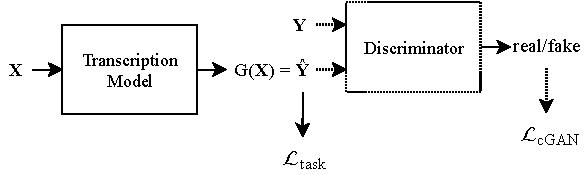
\includegraphics[width=0.8\columnwidth]{discriminator.pdf}
	\caption{A computation graph showing how a discriminator is appended to the original model. The appended parts are shown as dotted components.}\label{fig:discriminator}
\end{figure}

Adversarial training with $\mathcal{L}_{\text{cGAN}}$ allows the model to learn the inter-label dependencies as desired, even when $\mathcal{L}_{\text{task}}$ is defined only in terms of element-wise operations between $\hat{\Y}$ and $\Y$, as in Equation \ref{eqn:elementwise}.
In the next subsection, we describe a neural network architecture for the  cGAN discriminator that leverages prior knowledge on music.


\subsection{Musically Inspired Adversarial Discriminator}

Following \texttt{pix2pix}, we use a fully convolutional architecture~\cite{long2015fcn} for the discriminator.
By being fully convolutional, the discriminator has translation invariance not only along the time axis (as in HMMs and RNNs) but also along the frequency axis.
Since the discriminator determines how realistic a polyphonic note sequence is, the translation invariance enforces that the decision does not depend on the musical key, but only on the relative pitch and time intervals between the notes.
This effectively implements a music language model (MLM)~\cite{boulangerlewandowski2012temporal,sigtia2016endtoend} and biases the transcription toward more realistic note sequences.

Unlike the image-to-image translation problem, the input representations (e.g.~Mel spectrograms) and the output representations (e.g.~piano rolls) of a music transcription model can have different dimensions.
This makes combining $\X$ and $\Y$ in a fully convolutional manner difficult.
For this reason, we make the discriminator a function of $\Y$ only, simplifying the objective in Equation \ref{eqn:cgan} to:
\begin{equation}\label{eqn:simple-cgan}
\mathcal{L}_{\text{cGAN}}(G, D) ~ = ~  \mathbb{E}_{\Y}  \log D(\Y) ~ + ~ \mathbb{E}_{\X} \log (1 - D ( G(\X))).
\end{equation}
Note that $\z$ is also omitted in Equation \ref{eqn:simple-cgan}, as we follow \cite{isola2017pix2pix} and implement the stochasticity of $\z$ only in terms of dropout layers \cite{srivastava2014dropout}, without explicitly feeding random noises into the generator.
This causes a mode collapse problem where the learned $p(\Y|\X)$ is not diverse enough, but it does not harm our purpose of producing more realistic target representations.

\subsection{TTUR and \textit{mixup} to Stabilize GAN Training}

Although an ideal GAN generator can fully reconstruct the data distribution at the global optimum~\cite{goodfellow2014gan}, training of GANs in practice is notoriously difficult, especially for high-dimensional data~\cite{goodfellow2016gan}.
This led to the inventions of a plethora of techniques for stabilizing GAN training, among which we employ the two-timescale update rule (TTUR)~\cite{heusel2017ttur} and \textit{mixup}~\cite{zhang2018mixup}.
TTUR means simply setting the generator's learning rate a few times larger than that of the discriminator, which has been empirically shown to stabilize GAN training significantly.

The other technique, \textit{mixup}, is an extension to empirical risk minimization where training data samples are drawn from convex interpolations between pairs of empirical data samples.
For a pair of feature-target tuples $(\X_i, \Y_i)$ and $(\X_j, \Y_j)$ sampled randomly from the empirical distribution, their convex interpolation is given by:
\begin{equation}
\begin{array}{l@{}l}
\tilde{\X} = \lambda \X_i + (1 - \lambda) \X_j \\
\tilde{\Y} = \lambda \Y_i + (1 - \lambda) \Y_j
\end{array}
\end{equation}
where $\lambda \sim \text{Beta}(\alpha, \alpha)$, and $\alpha$ is the \textit{mixup} hyperparameter which controls the strength of interpolation.
When $\alpha = 0$, the Beta distribution becomes $\text{Bernoulli}(0.5)$ which recovers the usual GAN training without \textit{mixup}.
%\TODO{a figure visualizing mixup}


\setlength{\algomargin}{0em}
\DontPrintSemicolon
\SetInd{0.1em}{2em}
\begin{algorithm2e}[b!]
	\vspace{-0.3em}\noindent
	\caption{Training of a \textit{mixup} Conditional GAN.}\label{alg:training}
	\setstretch{1.05}
	\rule{\columnwidth}{0.75pt}\\
	\KwIn{
		Generator $G_\vartheta(\X)$ with initial parameters $\vartheta$, learning rate $\eta$, and loss function $\mathcal{L}_{\text{task}}(\hat{\Y}, \Y)$, discriminator $D_\varphi(\Y)$ with initial parameters $\varphi$, learning rate $\beta$, and loss function $\ell \in \{\text{BCE}, \text{MSE}\}$, batch size $m$, training data distribution $p(\X, \Y)$,  \texttt{pix2pix} weight $\nu$, \textit{mixup} strength $\alpha$.
	}

	\KwOut{Trained conditional generator $G_\vartheta(\X)$.}
	\vspace{-0.5em}\noindent
	\rule{\columnwidth}{0.5pt}\\
	%\vspace{-1em}
	\While{$\varphi$ and $\vartheta$ have not converged}{
		$\{(\X_i, \Y_i)\}_{i=1,\cdots,m} \leftarrow m \text{ samples from } p(\X, \Y)$\;
		\For{$i = 1, \cdots, m$}{
			$\hat{\Y}_i \leftarrow G_\vartheta(\X_i)$\;
			$\lambda_i \leftarrow \text{sample from Beta}(\alpha, \alpha)$\;
			$\tilde{\Y}_i \leftarrow \lambda_i \Y_i + (1 - \lambda_i) \hat{\Y}_i$
		}
		$\mathcal{L}_{\text{cGAN}}^D\>\leftarrow \textstyle\sum_{i=1}^M \ell(D_\varphi(\tilde{\Y}_i), \lambda_i)$\;
		$\varphi \leftarrow \varphi - \beta \cdot \nabla_\varphi \mathcal{L}_{\text{cGAN}}^D $\;
		$\mathcal{L}_{\text{cGAN}}^G \leftarrow \textstyle\sum_{i=1}^M \ell (D_\varphi(\tilde{\Y}_i), 1 - \lambda_i) $\;
		$\vartheta \leftarrow \vartheta - \eta \cdot \textstyle\nabla_\vartheta \Big [ \sum_{i=1}^m \nu \mathcal{L}_{\text{task}}(\hat{\Y}_i, Y_i) - \mathcal{L}_{\text{cGAN}}^G \Big ] $
	}
	\vspace{-0.5em}\noindent
	\rule{\columnwidth}{0.75pt}\;
\end{algorithm2e}



\textit{mixup} is readily applicable to the binary classification task of GAN discriminators.
In our conditional GAN setup, we have an additional advantage of having paired samples of a real label $\Y$ and a fake label $\hat{\Y} = G(\X)$, which allow us to replace Equation \ref{eqn:simple-cgan} with:
\begin{equation}\label{eqn:mixup-gan}
\min_{G} ~ \max_{D} ~ \mathbb{E}_{\X,\Y,\lambda} \Big [ - \ell (D(\lambda \Y + (1 - \lambda) G(\X) ), ~ \lambda) \Big ].
\end{equation}
where $\ell(p, y) = - y \log p - (1-y) \log (1-p)$ is the binary cross entropy (BCE) function.
With this \textit{mixup} setup, the discriminator now has to operate on the convex interpolation between the predicted representation and the corresponding ground truth.
This makes the discriminator's task even more difficult when the prediction gets close to the ground truth, which is desirable because the discriminator should be inconclusive (i.e. $D = \tfrac{1}{2}$ everywhere) at the global optimum~\cite{goodfellow2014gan}.

Algorithm \ref{alg:training} details the procedure of training the conditional GAN using \textit{mixup}, based on Equations \ref{eqn:simple-cgan} and \ref{eqn:mixup-gan}.
Note that for training the generator network, we perform label flipping in $\mathcal{L}_{\text{cGAN}}^G$ similarly as in Equation \ref{eqn:nsgan}.
Also, to train a least-squares GAN (Equation \ref{eqn:lsgan}) instead, we can simply replace $\ell$ with a mean squared error (MSE) loss.


\begin{table}[t]
	\small
	\renewcommand\arraystretch{1.2}
	\renewcommand{\tabcolsep}{5pt}
	\centering
	\begin{tabular}{l c} \toprule
		Hyperparameter & Values \\ \hline
		Generator learning rate $\eta$ & 0.0006 \\ 
		Discriminator learning rate $\beta$ & 0.0001 \\
		Discriminator loss function $\ell$ & \{BCE, MSE\}\\
		Batch size $m$ & 8 \\
		\texttt{pix2pix} weight $\nu$ & 100 \\
		\textit{mixup} strength $\alpha$ & \{0, 0.2, 0.3, 0.4\} \\
		Activation threshold $\tau$ & 0.5 \\
		Training sequence length & 327,680 \\
		\bottomrule
	\end{tabular}
	\vspace{1em}
	\caption{Hyperparameters used during the experiments.}\label{tab:hyperparameters}
\end{table}

\begin{table}[t]
	\small
	\centering
	\renewcommand\arraystretch{1.5}
	\renewcommand{\tabcolsep}{0em}
	\newcolumntype{M}[1]{>{\centering\arraybackslash}b{#1}}
	\newcolumntype{C}{>{\centering\arraybackslash}m{2.4em}}
	\begin{tabular}{@{\extracolsep{1em}}lM{4em}M{8em}CCCC}
		& & & \multicolumn{4}{c}{\textit{mixup} strength $\alpha$} \\ \cline{4-7}
		& Baseline & GAN type & 0 & 0.2 & 0.3 & 0.4 \\ \hline
		\multirow{2.25}{5em}{Frame F1} & \multirow{2.25}{4em}{\centering0.899} & Non-Saturating & 0.664 & 0.912 & \textbf{0.914} & 0.907 \\
		& & Least-Squares & 0.904 & 0.903 & 0.906 & 0.898 \\ \hline
		\multirow{2.25}{5em}{Note F1} & \multirow{2.25}{4em}{\centering0.942} & Non-Saturating & 0.717 & 0.953 & \textbf{0.956} & 0.951 \\
		& & Least-Squares & 0.944 & 0.947 & 0.950 & 0.943 \\
		\hline
	\end{tabular}
	\vspace{1em}
	\caption{Frame and note F1 scores are the highest when the non-saturating GAN loss and $\alpha = 0.3$ are used.}\label{tab:alpha}
\end{table}

\begin{table*}[t]
	\centering
	\footnotesize
	\renewcommand\arraystretch{1.5}
	\renewcommand{\tabcolsep}{0em}
	\newcolumntype{M}[1]{>{\centering\arraybackslash}b{#1}}
	\newcolumntype{C}{>{\centering\arraybackslash}m{4em}}
	\begin{tabular}{@{\extracolsep{0.5em}}llllCCCCCCC}
		& & & &\multirow{3.3}{4em}{\centering Baseline} &\multicolumn{3}{M{13em}}{\centering Non-Saturating GAN}
		&\multicolumn{3}{M{13em}}{\centering Least-Squares GAN} \\
		\cline{6-8} \cline{9-11}
		& & & & & $\alpha = 0.2$ & $\alpha = 0.3$ & $\alpha = 0.4$ & $\alpha = 0.2$ & $\alpha = 0.3$ & $\alpha = 0.4$ \\ \hline
		\parbox[t]{2mm}{\multirow{7.4}{*}{\rotatebox[origin=c]{90}{Frame Metrics}}} & & & F1 & 0.899 & 0.912 & \textbf{\small0.914} & 0.907 & 0.901 & 0.906 & 0.898 \\
		& & & Precision ~~~ & 0.946 & 0.937 & 0.931 & 0.939 & 0.940 & 0.942 & 0.946 \\
		& & & Recall & 0.857 & 0.889 & 0.898 & 0.879 & 0.865 & 0.875 & 0.855 \\
		& & & $E_\text{total}$ & 0.179 & 0.157 & 0.156 & 0.166 & 0.176 & 0.167 & 0.181 \\
		& & & $E_\text{subs}$ & 0.013 & 0.013 & 0.012 & 0.013 & 0.014 & 0.013 & 0.013 \\
		& & & $E_\text{miss}$ & 0.130 & 0.097 & 0.089 & 0.108 & 0.121 & 0.113 & 0.132 \\
		& & & $E_\text{fa}$ & 0.036 & 0.047 & 0.054 & 0.045 & 0.042 & 0.042 & 0.036 \\ \hline
		\parbox[t]{2mm}{\multirow{3.2}{*}{\rotatebox[origin=c]{90}{Note}}} & & & F1 & 0.942 & 0.953 & \textbf{\small0.956} & 0.951 & 0.944 & 0.950 & 0.941 \\
		& & & Precision & 0.990 & 0.974 & 0.981 & 0.973 & 0.986 & 0.988 & 0.989 \\
		& & & Recall & 0.899 & 0.933 & 0.932 & 0.930 & 0.905 & 0.916 & 0.898 \\ \hline
		\parbox[t]{2mm}{\multirow{3.2}{*}{\rotatebox[origin=c]{90}{Note with}}} & \parbox[t]{2mm}{\multirow{3.2}{*}{\rotatebox[origin=c]{90}{Offsets}}} & & F1 & 0.802 & 0.811 & \textbf{\small0.813} & 0.799 & 0.799 & 0.810 & 0.798 \\
		& & & Precision & 0.842 & 0.828 & 0.835 & 0.817 & 0.835 & 0.841 & 0.838 \\
		& & & Recall & 0.765 & 0.794 & 0.793 & 0.782 & 0.767 & 0.781 & 0.762 \\ \hline
		\parbox[t]{2mm}{\multirow{3.2}{*}{\rotatebox[origin=c]{90}{Note with}}} & \parbox[t]{2mm}{\multirow{3.2}{*}{\rotatebox[origin=c]{90}{Offsets and}}} & \parbox[t]{4mm}{\multirow{3.2}{*}{\rotatebox[origin=c]{90}{Velocity}}} & F1 & 0.790 & 0.799 & \textbf{\small0.802} & 0.787 & 0.788 & 0.799 & 0.787 \\
		& & & Precision & 0.830 & 0.816 & 0.823 & 0.805 & 0.823 & 0.830 & 0.827 \\
		& & & Recall & 0.755 & 0.783 & 0.782 & 0.770 & 0.757 & 0.771 & 0.752 \\ \hline
	\end{tabular}
	\vspace{1em}
	\caption{Summary of transcription performance. The non-saturating GAN loss achieves the best performance across all F1 metrics. The average metrics across the tracks in the MAESTRO test dataset are reported, and the model checkpoint where the average of frame F1 and note F1 is the highest on the validation dataset is used.}\label{tab:performance}
\end{table*}


\section{Experimental Setup}

To verify the effectiveness of our approach, we compare Onsets and Frames~\cite{hawthorne2018onsetsframes}, a state-of-the-art piano transcription model, with variants of the same model that are trained with the adversarial loss.
We also aim to evaluate the choices of the GAN loss and the \textit{mixup} strength $\alpha$.

\subsection{Model Architecture}

We use the extended Onsets and Frames model~\cite{hawthorne2019maestro} which increased the CNN channels to 48/48/96, the LSTM units to 256, and the FC units to 768.
The extended model has a total of 26.5 million parameters.
We do not use the frame loss weights described in~\cite{hawthorne2018onsetsframes} in favor of the offset stack introduced in the extended version (see Figure~\ref{fig:onsetsframes}).
During inference, we first calculate the posteriors corresponding to overlapping chunks of audio, with the same length as the training sequences, and perform overlap-add (OLA) using Hamming windows to obtain the full-length posterior.
We perform OLA instead of applying the recurrent calculations for the full length, because the effects of adversarial learning are best achieved within the training sequence length.

The input to the discriminator has two channels for the onset and frame predictions.
The discriminator has 5 convolutional layers: \texttt{c32k3s2p1}, \texttt{c64k3s2p1}, \texttt{c128k3s2p1}, \texttt{c256k3s2p1}, \texttt{c1k5s1p2}, where the numbers indicate the number of output channels, the kernel size, the stride amount, and the padding size.
At each non-final layer, dropout of probability 0.5 and leaky ReLU activation with negative slope 0.2 are used.
The mean of the final layer output along the time and frequency axes is taken as the discriminator output.



\subsection{Hyperparameters}

Table \ref{tab:hyperparameters} summarizes the hyperparameters used during the experiments, which are mostly taken directly from~\citeA{hawthorne2018onsetsframes} and \citeA{isola2017pix2pix}.
Also following~\citeA{hawthorne2018onsetsframes}, we use Adam~\cite{kingma2015adam} and apply learning rate decay of factor 0.98 in every 10,000 iterations, for both the generator and the discriminator.
We examine two types of GAN losses, the non-saturating GAN ($\ell = \text{BCE}$) and the least-squares GAN ($\ell = \text{MSE}$).
For each GAN loss, multiple values of \textit{mixup} strengths are compared with $\alpha = 0$, i.e. no \textit{mixup}.
Training runs for one million iterations, and the iteration that best performs on the validation set are used for evaluation on the test set.

\subsection{Dataset}

We use the MAESTRO dataset~\cite{hawthorne2019maestro}, which contains Disklavier recordings of 1,184 classical piano performances.
The dataset consists of 172.3 hours of audio, which are provided with 140.1, 15.3, and 16.9 hours of train/validation/test splits such that recordings of one composition only appear in the same split.
We resample the audio to 16 kHz and down-mix into a single channel.
Following~\citeA{hawthorne2018onsetsframes}, an STFT window of 2,048 samples is used for producing 229-bin Mel spectrograms, and a hop length of 32 ms is used.
% We do not perform audio amplitude normalization on the dataset, following the official implementation.
Training sequences sliced at random positions are used, unlike the official implementation which slices training sequences at silence or zero crossings.

\subsection{Evaluation Metrics}

The Onsets and Frames model perform both frame-level and note-level predictions, and their performance can be evaluated with the standard precision, recall, and F1 metrics.
For multi-pitch estimation, we also report the error rate metrics defined by~\citeA{poliner2006discriminative}, which include total error, substitution error, miss error, and false alarm error.
We use the \texttt{mir\_eval}~\cite{raffel2014mir_eval} library for all metric calculations.
For the note-level metrics, we use the default settings of the library, which use 50 ms for the onset tolerance, 50 ms or 20\% of the note length (whichever is longer) for the offset tolerance, and 0.1 for the velocity tolerance.


\section{Results}

%Our results show that adversarial learning brings a consistent improvement over the baseline which is already very robust, as shown with quantitative and qualitative analyses in the following subsections.


\subsection{Comparison with the Baseline Metrics}

\begin{figure*}[t]
	\centering
	\minipage{1.03\textwidth}
	\hspace{-0.02\textwidth}
	\includegraphics[width=0.499\textwidth]{predictions-115.pdf}%
	\includegraphics[width=0.499\textwidth]{predictions-73.pdf}%
	%\includegraphics[width=0.333\textwidth]{predictions-64.pdf}%
	\endminipage
	\caption{Comparisons of the frame activation posterior predicted by the baseline and our model ($\ell = \text{BCE}$, $\alpha = 0.3$), on three example segments. The input Mel spectrograms and the target piano rolls are shown together. The GAN version produces more confident predictions compared to the noisy baselines, leading to more accurate predictions.}\label{fig:predictions}
\end{figure*}

\begin{figure*}[t]
	\centering
	\includegraphics[height=12em]{pertrack.pdf}
	\caption{Distribution of the F1 score improvements over the baseline, tested on the MAESTRO test tracks.}\label{fig:pertrack}
\end{figure*}
\begin{figure*}[t]
	\centering
	\includegraphics[height=12em]{distribution.pdf}
	\caption{Distribution of frame activation values. Our model outputs more confident predictions, as indicated by the lower relative frequency in (0.1, 0.9).}\label{fig:distribution}
\end{figure*}
\begin{figure*}[t]
	\centering
	\includegraphics[height=12em]{training.pdf}
	\caption{Learning curves showing the generalization gaps; training curves are drawn as dotted lines, and test curves are drawn as solid lines.}\label{fig:training}
\end{figure*}

Table \ref{tab:alpha} and \ref{tab:performance} summarize the transcription performance, clearly showing a consistent improvement in the conditional GAN models over the Onsets and Frames baseline.
Table \ref{tab:alpha} shows that both non-saturating GAN and least-squares GAN achieve the highest frame and note F1 scores when the \textit{mixup} strength $\alpha = 0.3$ is used, and they both outperform the baseline.
The binary piano rolls are easy to distinguish from the non-binary predictions, which may cause imbalanced adversarial training. \textit{mixup} allows non-binary piano rolls to be fed to the discriminator, making its task more challenging and leading to higher performance.

Table \ref{tab:performance} shows an important trend of the cGAN results compared to the baseline that cGAN trades off a bit of precision for a significant improvement in recall; this is a side effect of the cGAN producing more confident predictions, as will be discussed in the following subsections.

While the percentage differences are moderate, our method achieves statistically significant improvements in F1 metrics on the MAESTRO test dataset ($p < 10^{-14}$ for all 4 metrics, two-tailed paired $t$-test).
The distribution of per-track improvement in each F1 metric is shown in Figure \ref{fig:pertrack}, which indicates that the improvements are evenly distributed across the majority of the tracks.
These improvements are especially promising, considering that Onsets and Frames is already a very strong baseline.

\subsection{Visualization of Frame Activations}

To better understand the inner workings of the conditional GAN framework, we visualize the frame posteriorgrams created by the baseline and the best performing conditional GAN model in Figure \ref{fig:predictions}.
In contrast to the baseline posteriorgrams which have many blurry segments, the posteriorgrams generated by our method mostly contain segments with solid colors, meaning that the model is more confident in its prediction.
Figure~\ref{fig:distribution} shows that the proportion of frame activation values in $(0.1, 0.9)$ is noticeably higher in the baseline, thus making the output less sensitive to the threshold choice.
This is because indecisive predictions are penalized by the discriminator, since they are easy to distinguish from the ground-truth which contains only binary labels.
The generator is therefore encouraged to output the most probable note sequences even when it is unsure, rather than producing blurry posteriorgrams that might hamper the decoding process.
This allows for an interpretation in which the GAN loss provides a prior for valid onset and frame activations, and the model learns to perform MAP estimation based on this prior.


\subsection{Training Dynamics and The Generalization Gap}

Figure \ref{fig:training} shows the learning curves for the frame F1 and note F1 scores, where the scores on the training dataset are plotted in dotted lines.
It is noticeable in the figure that the validation F1 scores for the baseline stagnate after 300k iterations, while the F1 scores of our model steadily grow until the end of 1 million iterations.
Thanks to this, the generalization gap --- the difference between the training and validation F1 scores --- is significantly smaller for the conditional GAN model.
This means that the GAN loss works as an effective regularizer that encourages the trained model to generalize better to unseen data, rather than memorizing the note sequences in the training dataset as LSTMs are known to be capable of~\cite{zaremba2015recurrent}.

\section{Conclusions}

We have presented an adversarial training method that can consistently outperform the baseline Onsets and Frames model, using the standard frame-level and note-level transcription metrics and visualizations that show how the improved model predicts more confident output.
To achieve this, a discriminator network is trained competitively with the transcription model, i.e. a conditional generator, so that the discriminator serves as a learned regularizer that provides a prior for realistic note sequences.
After training, the discriminator can be disregarded for inference, incurring no additional computational cost during transcription.


Our results show that modeling the inter-label dependencies in the target distribution is important and brings measurable performance improvements.
Our method is generic, and any model that involves predicting two-dimensional representation should be able to benefit from including an adversarial loss.
These approaches are common not only in transcription models but also in speech or music synthesis models that predict spectrograms as an intermediate representation~\cite{shen2018tacotron,kim2019synthesis}.
This implies that the findings in this chapter is applicable to a broader set of problems not only in multi-pitch estimation but also in the field of music information retrieval in general.

Our results do not include the effects of using data augmentation~\cite{hawthorne2019maestro}, which is orthogonal to our approach and should bring additional performance improvements when applied.
As discussed, the discriminator imposes the prior on the target domain whereas data augmentation enriches the input audio distribution.
This implies that our method would be less effective when the majority of errors are due to the discrepancy in the audio distribution between the training and test datasets.
How to apply adversarial learning for better generalization on the input distribution is a potential future research direction.

We have argued that the adversarial discriminator serves as a regularizer providing the prior knowledge of how the note sequences in the dataset should look like, which complements the conditionally independent output of the Onsets and Frames model.
The fully-connected output layer also does not take into account a very important characteristic of pitch, that each pitch corresponds to quasi-periodic signals in the input with a known frequency that are geometrically spaced --- rather, the predictions are instead made as if each pitch is completely independent pieces of information, not utilizing the knowledge on pitch at all.
Another important concept that is not considered in this chapter is the timbre.
Although the MAESTRO dataset used in this chapter contains various recording conditions and therefore somewhat different timbres among the tracks, they are all recordings of piano performances which have limited timbral diversity.
These aspects motivate building an improved model that can leverage the regularity of pitch as well as the knowledge of instrumental timbres.
In the next chapter, we discuss how to extend our music transcription model to incorporate such aspects, specifically by using a synthesizer model similar to the one used in Chapter \ref{ch:synthesis}.


\setcounter{chapter}{6}
%!TEX root = ../dissertation.tex
% this file is called up by thesis.tex
% content in this file will be fed into the main document

\graphicspath{{7-timbre/figures/}}

\chapter{Synthesizer-Aided Multi-Instrument Transcription}
\label{ch:timbre}

In Chapter \ref{ch:introduction}, we introduced the idea of extending a music transcription model with an additional synthesizer component that can convert the transcribed information back to the input audio, forming an analysis/synthesis framework as depicted in the encoder-decoder architecture in Figure \ref{fig:autoencoder}.
By doing so, we anticipated that the two components --- the transcriber and the synthesizer --- can work together to better translate information between the two representations, i.e. audio waveform and the transcribed semantic information of the music.
One motivation for employing such analysis/synthesis framework is that the advent of many successful deep learning techniques and the improved hardware capability may allow us to convert an audio signal completely into the constituent pieces of musical information that we want to transcribe, that are entangled in an extremely sophisticated way in the audio signal.
In the preceding chapters, we have considered deep learning solutions to various problems in music analysis and synthesis, such as monophonic pitch tracking (Chapter \ref{ch:monophonic}), music synthesis with controllable timbre (Chapter \ref{ch:synthesis}), and polyphonic music transcription (Chapter \ref{ch:adversarial}).
These problems correspond to a certain subset of the full encoder-decoder architecture, and in each chapter we discussed how the design choices in the model architecture and dataset construction affect the experimental results and the real-world applicability.

Having learned the lessons from these, in this chapter we aim to construct an automatic music transcription system that encompasses the full analysis/synthesis cycle, by considering the general problem of multi-instrument polyphonic music transcription.
We propose an autoencoder architecture that appends a synthesis model on top of a transcription model, and we verify the effects of the appended synthesizer in the experiments.
As in Chapter \ref{ch:synthesis}, the synthesizer component is capable of capturing the different aspects of various timbres in the dataset using a learned timbre space representation.
We show that the synthesizer component can serve as a regularizer to the transcriber, providing a form of prior knowledge on the spectral and temporal characteristics of the timbres. 
% \TODO{some conclusive sentence summarizing the results of this chapter}

\section{Introduction}

Multi-instrument music transcription aims to extract not only the occurrences of multiple simultaneous pitches and notes but also the types of one or more instruments corresponding to those notes.
Since it poses additional challenges to the already difficult problem of polyphonic music transcription, studies on the complete multi-instrument polyphonic transcription problem are relatively rare.
Instead, most studies on analyzing multi-instrument audio focus on either developing a discriminative model for polyphonic where timbre information is disregarded~\cite{bittner2017deepsalience} %\TODO{cite more}
or the problem of instrument recognition, while not identifying the individual notes that belongs to the recognized instruments~\cite{lostanlen2016spiral}. %\TODO{cite more}
To take both polyphonic notes and multiple instruments into account, a model has to carefully incorporate the prior knowledge of how pitch and timbre are reflected in the audio signal, e.g. using a probabilistic latent component model~\cite{benetos2015probabilistic} or a variant of non-negative matrix factorization~\cite{grindlay2009eigeninstruments}.
To produce outputs in multiple domains, these models have to include an intricate set of design choices to implement a mathematical representation of the prior knowledge.

Meanwhile, the main premise of deep learning is quite opposite of how those models are designed.
Rather than writing down the set of rules manually, layers of simple calculations can serve as a very effective function approximator, that can produce just about anything when an enough amount of data is fed to the black box.
In these models, the prior knowledge baked into the model architecture is minimal.
Take the Onsets and Frames model~\cite{hawthorne2018onsetsframes} for example; the model output has 88 dimensions corresponding to each key of the piano, but the 88 keys are treated as a separate multi-label target, without utilizing the knowledge that each key should represent a certain frequency that the quasi-periodic signal in the input follows.
Because of this lack of ``inductive bias'', deep learning models typically have to be trained with a very large amount of data; in other words, they are less sample efficient.


Generative models for transcription, such as a Bayesian network representation of spectrogram~\cite{bergkirkpatrick2014unsupervised}, takes the opposite approach.
These models define the process of generating sound entirely from the parameterized sources that typically convey a physical interpretation, such as the modeling of attack-decay-sustain-release (ADSR) curves or the energy distribution along harmonics. 
Compared to data-driven models with a lot of learnable parameters, however, those interpretable transcription models often lack the flexibility to be applicable for a wider variety of inputs.

In this chapter, we explore the possibility of finding a compromise between the two extremes.
Specifically, we examine how to induce the transcription model to make predictions such that, when synthesized back into audio, resemble the original audio input.
We do this by appending a neural music synthesis model to the transcription model, and the synthesis model is specifically designed to describe the sound generation process with a small number of interpretable parameters, which is restrictive enough to guide the transcription model to more accurate predictions, yet flexible enough to be learnable in a data-driven manner.
We evaluate this approach with a multi-instrument transcription task and show that a synthesis model can serve as an effective regularizer. % \TODO{describe qualitative improvement}

\section{Background}


\subsection{Multi-Instrument Music Transcription}

\cite{itoyama2011bayesian}: instrument recognition, \TODO{add more; interconnected with source separation}

\cite{grindlay2009eigeninstruments}: Hierarchical eigeninstruments

\cite{benetos2015probabilistic}: Probabilistic model (PLCA), spectral template, EM maximization

\cite{thickstun2017musicnet}: MusicNet, \cite{thickstun2018invariances} invariances,

\subsection{Deep Clustering}

\cite{hershey2016deepclustering}

\subsection{Source-Filter Synthesis}

\cite{heittola2009separation} (instrument recognition)

\subsection{Synthesizer Component for Transcription}

\citeA{li2017infinite} explored the idea of using on-the-fly synthesized training dataset for piano transcription, using a simple fully-connected neural network operating on the CQT representation.
The idea of using generative models to predict multiple fundamental frequencies is also not new \cite{dubois2005harmonic,cemgil2006generative}, but the authors relied on manually designed generative models for sound generation, which limits the expressibility and the generalizability of the model.
Using deep generative models can be a direction for overcoming these limitations, since the recent neural network approaches for audio generation are capable of producing highly realistic sounds.

\cite{choi2019drum} \cite{bergkirkpatrick2014unsupervised}


\section{Method}

We first describe the synthesizer model, followed by the modifications to the Onsets and Frames~\cite{hawthorne2018onsetsframes} transcription model made to allow the concatenation of the two models.

\subsection{Synthesizer Model}

The synthesizer model takes a per-instrument piano roll representation of symbolic music (see Figure \ref{fig:transcription-to-piano-rolls}) and uses a learned instrument embedding to predict the Mel spectrogram of the corresponding audio.
We are assuming here that predicting Mel spectrograms is equivalent to synthesizing the audio for our purposes, since we have seen in Chapter \ref{ch:synthesis} that Mel spectrograms contain most of the perceivable information present in the audio content, and the original audio can readily be reconstructed using sample-based synthesis models like WaveNet~\cite{oord2016wavenet}.

The synthesizer consists of two subcomponents, the envelope estimator and the waveshaper, respectively implementing the temporal and spectral characteristics of the sound being synthesized.
The computation in each subcomponent is performed independently for each pitch-instrument combinations, and their results are combined to obtain the resulting Mel spectrogram, as shown in Figure \ref{fig:synthesizer-architecture}.
Both components take the instrument embedding in order for the synthesized audio to exhibit different temporal and spectral behaviors depending on the instrument, and together they ensure that the synthesis model only creates harmonic sounds with the frequency corresponding to the pitch of input notes and the spectral envelope consistent among each instrument.

The envelope estimator component predicts the temporal envelope of each note, by mapping the note activities into a latent space using a one-dimensional convolution layer, followed by a FiLM layer~\cite{perez2018film} to condition on the instrument.
A GRU layer~\cite{cho2014seq2seq} is then applied in order to model the temporal behavior, such as the attack-decay-sustain-release (ADSR) curves.
Meanwhile, the waveshaper component performs a subtractive synthesis to obtain the spectrum corresponding to each pitch and instrument.
We use two types of source waves, sawtooth and triangular, to make it easily adaptable to the timbres that primarily consists of odd harmonics, such as the clarinet.
The instrument embedding is used to predict the transfer function in the Mel frequency domain to be applied to each source spectrum, which is modeled as a polynomial function mapping Mel frequencies to log magnitudes.
The Mel spectrogram corresponding to each note can then be calculated in the complex domain, by assigning a random initial phase to each pitch-instrument pair and multiplying the temporal envelope predicted by the envelope estimator.
All of the per-note Mel spectrograms are then added to obtain the final Mel spectrogram output.



\begin{figure}
	\centering
	\includegraphics[width=\textwidth]{synthesizer-architecture.pdf}
	\caption{The synthesizer architecture. The temporal and spectral characteristics of each notes are respectively modeled by the envelope estimator and the waveshaper. This structure enforces each instrument to have consistent spectral and temporal envelopes across the pitch.}\label{fig:synthesizer-architecture}
\end{figure}


\subsection{Training Transcriber with Appended Synthesizer}

To append the synthesizer component to the output of the transcription model while keeping the full model differentiable, we expand the fully-connected layer predicting the frame activation to additionally predict the instrument embedding corresponding to each time-frequency bin.
Using the expanded outputs, the frame activations and the predicted embedding can be fed to the synthesizer component.
The frame activations are binarized before feeding to the synthesizer, and we use a gradient-stop for this connection.

The synthesizer model is separately trained, and the transcriber model is then optimized to minimize the sum of three losses:
\begin{equation}
\mathcal{L}_{\text{Overall}} = \mathcal{L}_{\text{Onsets \& Frames}} + \lambda \left ( \mathcal{L}_{\text{Embedding}} + \mathcal{L}_{\text{Synthesizer}} \right )
\end{equation}
The first term, $\mathcal{L}_{\text{Onsets \& Frames}}$, is the loss of the Onsets and Frames model which is the sum of the binary cross entropy of the onsets, offsets, and frame predictions.
We define $\mathcal{L}_{\text{Embedding}}$ as the mean squared error (MSE) between the predicted instrument embedding and the ground truth, and $\mathcal{L}_{\text{Synthesizer}}$ is defined as the mean cosine distance between the predicted and the ground-truth Mel spectra:
\begin{equation}
\mathcal{L}_{\text{Synthesizer}} = \mathbb{E}_{\hat{\mathbf{s}}, \mathbf{s}} \left [ 1 - \frac{ \hat{\mathbf{s}} \cdot \mathbf{s} }{\lVert \hat{\mathbf{s}} \rVert \lVert \mathbf{s} \rVert} \right ]
\end{equation}
where $\mathbf{s}$ follows the distribution of Mel spectra in the input audio, and $\hat{\mathbf{s}}$ is the Mel spectra predicted by the synthesizer based on the transcription predicted from $\mathbf{s}$.

\section{Experimental Setup}

We use the MusicNet dataset~\cite{thickstun2017musicnet} to train both the synthesizer and the transcriber.
The dataset contains 2,048 minutes of classical chamber music audio and labels, which comprises 330 recordings of various ensembles.
The dataset contains annotations of 11 General MIDI instruments: Acoustic Grand Piano, Harpsichord, Violin, Viola, Cello, Contrabass, French Horn, Oboe, Bassoon, Clarinet, and Flute.
Different recordings in the dataset have drastically different tuning, ranging more than a semitone in some recordings which would result in a wrong transcription even by a perfect transcriber.
To alleviate this, we preprocess the dataset by running a tuning estimator implemented in librosa~\cite{mcfee2015librosa} on each track and pitch-shifted any recordings that are more than 20 cents apart from the A440 tuning.

Unlike in Chapter~\ref{ch:adversarial}, we use the original Onsets and Frames model size of 512, and the transcription model contains 10 million parameters.
We use a 2-dimensional instrument embedding space to represent the distribution of the 11 instruments, and the polynomial transfer functions used in the subtractive synthesis are modeled by cubic B\'{e}zier curves.


The audio is resampled to 16kHz, and a training batch is composed of eight 20-second audio segments and labels.
We use Adam optimizer~\cite{kingma2015adam} with learning rate 0.0006, and the learning rate decay of factor 0.98 is applied every 1000 steps.
We ran the optimization for 180,000 steps and report the transcription accuracy evaluated on the 10 test recordings provided in the MusicNet dataset.

\section{Results}

\subsection{Synthesizer Output}

\subsection{Transcription Accuracy}

\subsection{Multi-Instrument Transcription}

\begin{itemize}
	\item Trained Synthesizer
	\item Transcription Metrics
	\item Multi-instrument
\end{itemize}

\subsection{MusicNet Inspector}



\section{Conclusion}

\begin{itemize}
	\item Discussion points: unison, dot product space, Lipschitz; volume information
\end{itemize}



\setcounter{chapter}{7}
%!TEX root = ../dissertation.tex
% this file is called up by thesis.tex
% content in this file will be fed into the main document

\graphicspath{{8-conclusions/figures/}}

\chapter{Conclusions and Final Remarks}
\label{ch:conclusions}

\section{Summary and Takeaways}

\begin{itemize}
	\item Dataset matters (highly correlated than images ~\cite{thickstun2018invariances})
	\item Prior knowledge matters in all domains
\end{itemize}


\section{Future Research Directions}

\begin{itemize}
	\item fully-fledged synthesis model
	\item sound as discrete events / sound atoms~\cite{leveau2008atoms}
	\item language model, unsupervised training \cite{huang2018transformer}
	\item Unlimited source of generated model
\end{itemize}


\subsection{A Turing Test for Automatic Music Transcription}

Finally, a consideration is needed for the fundamental limitation on any music transcription task, either automatic or manual, and when it can be said that AMT is solved.
Polyphonic music contains a mixture of sounds with an indefinite number of notes being played simultaneously; even the most experienced musicians may not be able to identify every note, and the audio mixture may not contain the sufficient information to convey all notes in the first place.
It would be unreasonable to expect anyone to perfectly transcribe all notes in the score of an orchestral music from an audio file, but it would be sensible for a trained musician to produce a version of score that, when played by the same orchestra, sounds indistinguishable to the original recording.
Considering these limitations, passing this ``transcriptional Turing test'' as shown in Figure \ref{fig:turing}, rather than achieving the 100\% accuracy on a certain dataset, should be the ultimate goal of automatic music transcription, at which point it can be said to have a human-level intelligence on this task.

\begin{figure}
	\includegraphics[width=\textwidth]{turing.pdf}
	\caption{The \emph{transcriptional Turing test}, to test whether an automatic music transcription algorithm has reached human-level. While this provides some conceptual insights to the adversarial training setup, to be covered in the later chapters, fully achieving the human-level performance is out of scope of this thesis.}
	\label{fig:turing}
\end{figure}

\section{Conclusions}

\pagebreak


%: ----------------------- bibliography ------------------------
{
\hypersetup{linkcolor = RoyalBlue}
\onehalfspacing
\renewcommand\bibliographytypesize{\small}
\bibliography{library/library}
}

%: ----------------------- appendices --------------------------
% \appendixbegin
% \include{backmatter/appendices}

%: --------------------------- index ---------------------------
% \clearpage
% \begin{footnotesize}
% \cleardoublepage % ensure the right page
% \phantomsection % sets an anchor
% \printindex
% \end{footnotesize}

\end{document}
